\documentclass{article}
\usepackage{amsmath,amssymb,amsfonts}
\usepackage{geometry}
\usepackage{hyperref}
\usepackage[ruled,vlined]{algorithm2e}
\usepackage{booktabs}
\usepackage{tabularx}
\usepackage{enumitem}
\usepackage{xcolor}
\usepackage[most]{tcolorbox}
\usepackage{tikz}
\usetikzlibrary{positioning, arrows.meta, calc, fit, backgrounds, shadows.blur}
\geometry{a4paper, margin=1in}

\newcommand{\code}[1]{\texttt{\small #1}}
\newcommand{\textftol}{\tau_{\mathrm{ftol}}}
\newcommand{\textstag}{\tau_{\mathrm{stag}}}
\newcommand{\textxtol}{\tau_{\mathrm{xtol}}}
\newcommand{\ftolinner}[1]{\tau^{\,\mathrm{inner}}_{\mathrm{ftol},#1}}

% --- Extension highlighting ---------------------------------------------
\definecolor{extcolor}{rgb}{0.00,0.35,0.70}
\newcommand{\ext}[1]{{\color{extcolor}\textbf{[ext]}\ #1}}
\newcommand{\extline}[1]{{\color{extcolor}#1}}

% --- Module-interface card ---------------------------------------------
% A small grey box rendered immediately above each algorithm declaration.
% Arguments: 1=called by, 2=calls, 3=inputs, 4=outputs.
\newtcolorbox{interfacecard}{
    colback=gray!5, colframe=gray!55, boxrule=0.4pt, arc=2pt,
    left=8pt, right=8pt, top=4pt, bottom=4pt,
    width=\textwidth, before skip=4pt, after skip=2pt
}
\newcommand{\moduleinterface}[4]{%
\begin{interfacecard}
\footnotesize
\begin{tabular}{@{}r@{\quad}p{0.82\textwidth}@{}}
\textit{Called by:} & #1 \\
\textit{Calls:}     & #2 \\
\textit{Inputs:}    & #3 \\
\textit{Outputs:}   & #4 \\
\end{tabular}
\end{interfacecard}
}

% Diagram styling
\tikzset{
    modnode/.style    = {draw, rounded corners=3pt, align=center, font=\small,
                         inner sep=5pt, fill=blue!8, drop shadow={opacity=0.2,
                         shadow xshift=0.5pt, shadow yshift=-0.5pt}},
    leafnode/.style   = {modnode, fill=blue!5},
    extnode/.style    = {modnode, fill=extcolor!10, draw=extcolor!70},
    edge/.style       = {-{Stealth[scale=0.9]}, thick, gray!70},
    edgelbl/.style    = {font=\scriptsize\itshape, fill=white, inner sep=1pt},
}

\hypersetup{
    colorlinks=true,
    linkcolor=black,
    urlcolor=black,
    citecolor=black
}

\title{Algorithmic Structure of the Stabilized Porous Navier--Stokes Solver}
\author{Antigravity AI \and Project Authors}
\date{\today}

\begin{document}
\maketitle

\begin{abstract}
\sloppy
This document specifies the nonlinear solver pipeline that drives a
single invocation of \code{run\_simulation} in the stabilized porous
Navier--Stokes solver. The pipeline is presented as a strict module
hierarchy: at the top sits the orchestrator (Algorithm O), which calls
two mid-level routines (Algorithms B and C, the Stage I and Stage II
solvers), each of which in turn invokes a shared Newton kernel
(Algorithm A), which is itself composed of three leaf primitives
(Algorithms A.1, A.2, A.3). A graphical map of this hierarchy is given
in Section~\ref{sec:tree}. Each algorithm is documented in two parts:
a brief \emph{interface card} listing its callers, callees, inputs and
outputs; and a procedural pseudocode box.

The presentation is organised in two strict tiers. Part~\ref{part:core}
describes the \emph{core algorithm}. Part~\ref{part:ext} documents two
\emph{optional extensions} that augment the core algorithm in specific
settings: a plateau verifier based on the Method of Manufactured
Solutions, which fires only when a candidate exact solution is supplied;
and a parameter-sweep harness that re-tunes a small number of
tolerances on a per-case basis. The two tiers are kept strictly
separate: passages and algorithm-line additions belonging to the
extensions are typeset in \extline{this colour} throughout.
\end{abstract}

\tableofcontents

% ============================================================
\part{The Core Algorithm}
\label{part:core}
% ============================================================

\section{Overview and Algorithmic Challenges}
\label{sec:overview}

The continuous problem is the stationary, incompressible, generalized
porous Navier--Stokes system on a domain $\Omega \subset \mathbb{R}^d$,
\begin{equation}
    \label{eq:strong}
    \begin{aligned}
    \boldsymbol{u} \cdot \nabla \boldsymbol{u}
        - \nabla \cdot (2 \nu \nabla^{\mathrm{s}} \boldsymbol{u})
        + \sigma(\alpha, \boldsymbol{u}) \boldsymbol{u}
        + \nabla p
        &= \boldsymbol{f}, \\
    \nabla \cdot \boldsymbol{u} &= 0,
    \end{aligned}
\end{equation}
discretised by an equal-order Lagrangian pair $(\boldsymbol{V}_h, Q_h)$
of degree $(k_v, k_p) = (k, k)$ and stabilised by a Variational
Multiscale (VMS) formulation. The drag tensor
$\sigma(\alpha, \boldsymbol{u}) = a(\alpha) + b(\alpha) |\boldsymbol{u}|$
couples the Darcy--Forchheimer regime to the convective momentum
balance; the porosity field $\alpha$ varies in space, and the
high-$\mathrm{Re}$, high-$\mathrm{Da}$ regimes the solver must handle
are exactly those in which the system becomes simultaneously
convection-dominated, reaction-dominated, and stiff.

\paragraph{Nonlinearity from convection and Forchheimer drag.}  Newton's
method converges quadratically once the iterate enters its quadratic
basin, but locating that basin from an arbitrary initial guess is
non-trivial when both $\boldsymbol{u}\cdot\nabla\boldsymbol{u}$ and the
$|\boldsymbol{u}|$ factor in $\sigma$ amplify any error in
$\boldsymbol{u}$. The solver must detect divergence and respond---either
by shortening the step (line search), by switching to an iteration map
with a wider basin (Picard), or by aborting cleanly.

\paragraph{Implicit OSGS projection.}  In the Orthogonal Sub-Grid Scale
formulation the sub-grid component lives in the orthogonal complement
$\mathcal{X}_{h0}^{\perp}$ of the finite element space; in practice the
projection $\boldsymbol{\pi}_h \in \mathcal{X}_h$ of the strong residual
is computed, and the sub-grid scale is identified with
$(I-\Pi_h)\mathcal{R}$. The projection itself depends on
$U_h = (\boldsymbol{u}_h, p_h)$, so a fully monolithic Jacobian would
embed the Fr\'echet derivative of an $L^2$ projection operator. Rather
than carrying this dense block, the solver \emph{slaves}
$\boldsymbol{\pi}_h$ to the current iterate: every residual evaluation
re-projects $\boldsymbol{\pi}_h = \Pi(\mathcal{R}(U_h))$ via a cached
mass solve while the assembled Jacobian holds it frozen, so the primary
system is driven to its root by a single inexact-Newton solve rather
than an outer fixed point.

\paragraph{Architecture of the response.}  The architecture that emerges
is a two-stage cascade. \emph{Stage~I} drives the algebraic system to a
converged ASGS state, regardless of the final stabilization method
requested. \emph{Stage~II} either reports the ASGS state directly or,
when the user has selected OSGS, runs a single coupled Newton solve on
$U_h$---with $\boldsymbol{\pi}_h$ re-projected from the current iterate
at every evaluation---initialised at the Stage~I solution. The
outermost orchestration (Algorithm~\ref{alg:O}) wires all of these
together.

\begin{quote}
\itshape
ASGS is always run first; OSGS, when requested, refines the ASGS state
through a single coupled Newton solve whose residual re-projects
$\boldsymbol{\pi}_h$ at every evaluation.
\end{quote}

% ============================================================
\section{Module Hierarchy}
\label{sec:tree}

The algorithms below are organised in a strict call hierarchy. The
orchestrator (Algorithm~\ref{alg:O}) sits at the top and dispatches to
two stage solvers (Algorithms~\ref{alg:B} and~\ref{alg:C}), both of
which build on a single shared Newton kernel
(Algorithm~\ref{alg:A}). The Newton kernel itself is built from three
leaf primitives (Algorithms~\ref{alg:A1}, \ref{alg:A2}, \ref{alg:A3}).
Figure~\ref{fig:hierarchy} shows the full tree.

\begin{figure}[h]
\centering
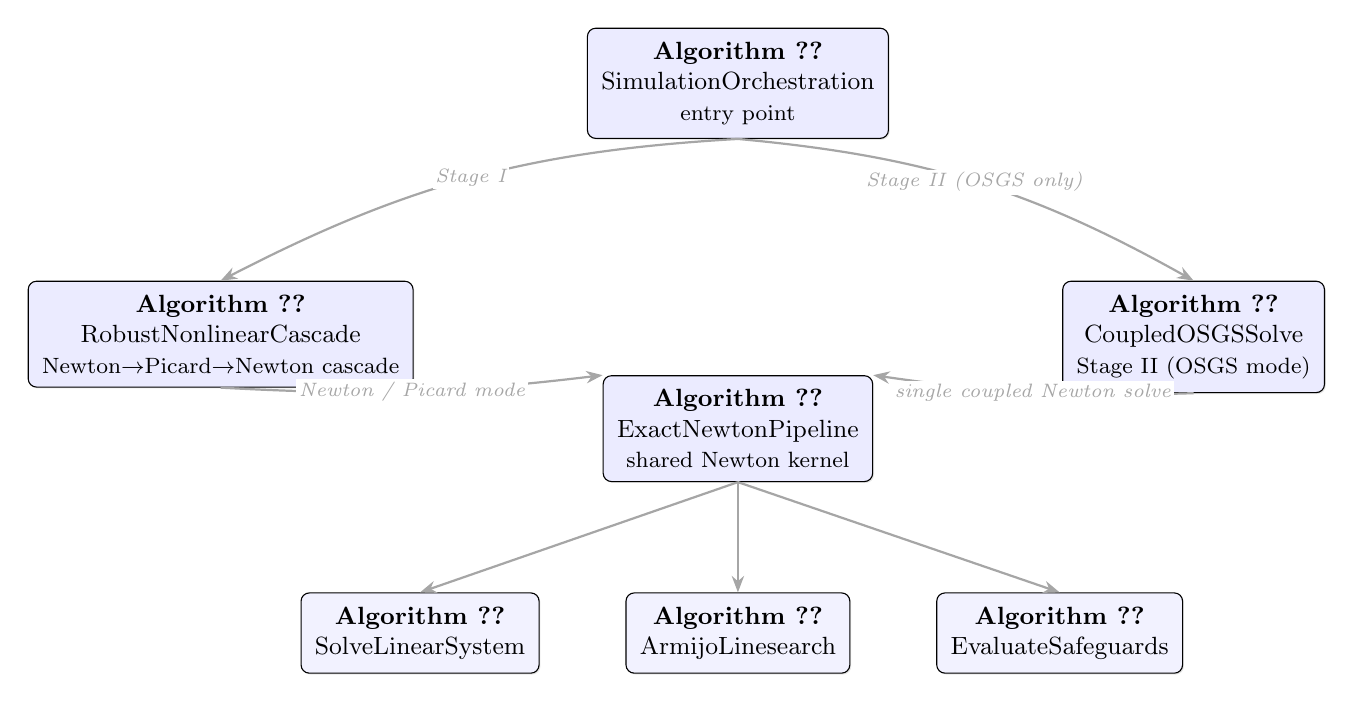
\begin{tikzpicture}[node distance=14mm and 10mm]

\node[modnode] (O)
    {\textbf{Algorithm~\ref{alg:O}}\\$\mathrm{SimulationOrchestration}$\\
     \footnotesize entry point};

\node[modnode, below left=18mm and 22mm of O] (B)
    {\textbf{Algorithm~\ref{alg:B}}\\$\mathrm{RobustNonlinearCascade}$\\
     \footnotesize Newton$\to$Picard$\to$Newton cascade};

\node[modnode, below right=18mm and 22mm of O] (C)
    {\textbf{Algorithm~\ref{alg:C}}\\$\mathrm{CoupledOSGSSolve}$\\
     \footnotesize Stage~II (OSGS mode)};

\node[modnode, below=30mm of O] (A)
    {\textbf{Algorithm~\ref{alg:A}}\\$\mathrm{ExactNewtonPipeline}$\\
     \footnotesize shared Newton kernel};

\node[leafnode, below left=14mm and 8mm of A] (A1)
    {\textbf{Algorithm~\ref{alg:A1}}\\$\mathrm{SolveLinearSystem}$};
\node[leafnode, below=14mm of A] (A2)
    {\textbf{Algorithm~\ref{alg:A2}}\\$\mathrm{ArmijoLinesearch}$};
\node[leafnode, below right=14mm and 8mm of A] (A3)
    {\textbf{Algorithm~\ref{alg:A3}}\\$\mathrm{EvaluateSafeguards}$};

\draw[edge] (O.south) to[bend right=12]
    node[edgelbl, midway] {Stage~I} (B.north);
\draw[edge] (O.south) to[bend left=12]
    node[edgelbl, midway] {Stage~II (OSGS only)} (C.north);
\draw[edge] (B.south) to[bend right=5]
    node[edgelbl, midway, fill=white] {Newton / Picard mode} (A.north west);
\draw[edge] (C.south) to[bend left=5]
    node[edgelbl, midway, fill=white] {single coupled Newton solve} (A.north east);
\draw[edge] (A.south) -- (A1.north);
\draw[edge] (A.south) -- (A2.north);
\draw[edge] (A.south) -- (A3.north);

\end{tikzpicture}
\caption{Module hierarchy of the core algorithm. Arrows point from
caller to callee. Each edge is annotated with the calling context.
Algorithm~\ref{alg:A} is the shared workhorse: Algorithm~\ref{alg:B}
(Stage~I) invokes it three times in sequence (Newton, then Picard, then
Newton) with different Jacobians, while Algorithm~\ref{alg:C} (Stage~II,
OSGS) invokes it once as a single coupled Newton solve whose residual
re-projects $\boldsymbol{\pi}_h$ at every evaluation. Leaf primitives
A.1--A.3 are pure procedures with no further dependencies.}
\label{fig:hierarchy}
\end{figure}

\paragraph{Code map.}  The source mirrors this tree:
Algorithm~\ref{alg:A} (the shared Newton kernel) is \code{src/solvers/nonlinear.jl};
Algorithms~\ref{alg:B} and~\ref{alg:O} (the Stage-I ASGS boot and the orchestrator) are
\code{src/solvers/asgs\_solver.jl}; Algorithm~\ref{alg:C} (the coupled OSGS solve,
\code{solve\_osgs\_stage!}) is \code{src/solvers/osgs\_solver.jl}; and the optional Algorithm~\ref{alg:D}
(\code{VerifyMMSPlateau}) is \code{src/solvers/mms\_verification.jl}, plugged in behind the
\code{SolutionVerifier} seam (\code{on\_asgs\_converged!} / \code{on\_osgs\_converged!}) so the production
path runs a no-op \code{NoVerification}.

\paragraph{Reading order.}  This document presents the modules
top-down: first the orchestrator (§\ref{sec:orchestration}), then the
two stage solvers (§\ref{sec:picard}, §\ref{sec:osgs}), then the shared
Newton kernel and its leaves (§\ref{sec:newton}). Each algorithm is
introduced by a short \emph{interface card} that summarises its
position in the tree---callers, callees, inputs, outputs---before the
procedural box. Mathematical preliminaries shared by several algorithms
(the diagonally equilibrated merit function and its directional
derivative identity) are gathered in §\ref{sec:math-prelim}.

% ============================================================
\section{Parameter Taxonomy and Code Equivalence}
\label{sec:params}

\subsection{Numerical parameters of the core algorithm}

Table~\ref{tab:params} enumerates every numerical parameter consumed by
the algorithms of Part~\ref{part:core}, grouped by role. Parameters
that belong to the optional extensions of Part~\ref{part:ext} are
tabulated separately in the corresponding sections.

\begin{table}[h]
\centering
\caption{Numerical parameters of the core nonlinear-solver pipeline.
Throughout the table, $\code{sol} = \code{config.numerical\_method.solver}$
(a flat \code{SolverConfig} \code{@kwdef} struct) and
$\code{stab} = \code{config.numerical\_method.stabilization}$. The
\code{SafeNewtonSolver} struct that runs the inner cascade is built from
these fields by \code{SafeNewtonSolver(::LinearSolver, ::SolverConfig)};
its post-construction field names (e.g.\ \code{c1}, \code{max\_iters})
are shorter aliases of the config field names. Code-side references in
this table are written against the config struct, not the built solver.}
\label{tab:params}
\footnotesize
\begin{tabularx}{\textwidth}{@{} l l X @{}}
\toprule
\textbf{Symbol} & \textbf{Field in code} & \textbf{Role / effect} \\
\midrule
\multicolumn{3}{l}{\emph{Inner Newton iteration controls}} \\
$N_{\mathrm{N}}$         & \code{sol.newton\_iterations}           & Cap on inner Newton iterations. \\
$N_{\mathrm{P}}$         & \code{sol.picard\_iterations}           & Cap on Picard fallback iterations. \\
$N_{\mathrm{inc}}$       & \code{sol.max\_increases}               & Consecutive merit-function expansions tolerated before declaring divergence. \\
$\textftol$              & \code{sol.ftol}                          & Terminal residual tolerance in $\ell^\infty$; the dominant convergence criterion. \\
$\textxtol$              & \code{sol.xtol}                          & Lower bound on the accepted step norm $\|\alpha\delta\boldsymbol{x}\|$ before declaring coordinate stagnation. \\
$\textstag$              & \code{sol.stagnation\_noise\_floor}      & Noise-floor residual; a non-converged exit below this may still be classified as success (Sec.~\ref{sec:falseEquiv}). \\
$\alpha_{\min}$          & \code{sol.linesearch\_alpha\_min}        & Smallest line-search step before giving up. \\
$c_1$                    & \code{sol.armijo\_c1}                    & Armijo / monotone-residual descent constant. \\
$\gamma$                 & \code{sol.linesearch\_contraction\_factor} & Backtracking factor: $\alpha \leftarrow \gamma\alpha$. \\
$N_{\mathrm{ls}}$        & \code{sol.max\_linesearch\_iterations}   & Bound on line-search inner iterations. \\
$F_{\mathrm{div}}$       & \code{sol.divergence\_merit\_factor}     & Threshold by which the merit must expand to count as one ``increase''. \\
$\mathfrak{m}$           & (built into the \code{SafeNewtonSolver} as \code{.mode})  & Cascade mode: \code{:newton} (merit-Armijo) or \code{:picard} (monotone residual reduction); cf.\ §\ref{sec:dir-deriv} and Alg.~\ref{alg:A2}. \\
\code{freeze\_cusp} & \code{sol.freeze\_jacobian\_cusp}   & Boolean: skip Jacobian recomputation at Forchheimer cusps to avoid singular updates. \\
\midrule
\multicolumn{3}{l}{\emph{OSGS coupled solve}} \\
$N_{\mathrm{OSGS}}$      & \code{stab.osgs\_iterations}             & Inner-Newton iteration cap for the single coupled OSGS solve (Alg.~\ref{alg:C}); the projection $\boldsymbol{\pi}_h$ is re-slaved every residual evaluation, so there is no separate outer-loop budget or drift criterion. \\
\bottomrule
\end{tabularx}
\end{table}

\subsection{Algorithm--to--code correspondence}

\begin{table}[h]
\centering
\caption{Algorithm $\leftrightarrow$ code signature mapping (core algorithm).}
\label{tab:functions}
\small
\begin{tabularx}{\textwidth}{@{} l X @{}}
\toprule
\textbf{Algorithm} & \textbf{Code entry point} \\
\midrule
$\mathrm{SimulationOrchestration}$ (Alg.~\ref{alg:O})   & \code{run\_simulation(path)} $\to$ \code{solve\_system(setup, form, solvers, cfg, x0)}. \\
$\mathrm{RobustNonlinearCascade}$ (Alg.~\ref{alg:B})    & The Newton$\to$Picard$\to$Newton cascade inside \code{solve\_system}; used only by Stage~I, the ASGS algebraic boot (\code{\_initialize\_asgs\_state!}, with ASGS operators and the restore vector $\boldsymbol{x}^0_{\mathrm{backup}}$). \\
$\mathrm{CoupledOSGSSolve}$ (Alg.~\ref{alg:C})  & The single coupled OSGS Newton solve inside \code{solve\_system}: one \code{safe\_fe\_solve!} call on Algorithm~\ref{alg:A} whose residual re-slaves $\boldsymbol{\pi}_h$ at every evaluation. \\
$\mathrm{ExactNewtonPipeline}$ (Alg.~\ref{alg:A})       & \code{\_safe\_solve\_inner!} (\code{src/solvers/nonlinear.jl}), reused with either an exact-Newton or a Picard Jacobian. \\
$\mathrm{SolveLinearSystem}$ (Alg.~\ref{alg:A1})        & \code{eval\_linear\_system\_resolution!(dx, A, b, solver, cache)}. \\
$\mathrm{ArmijoLinesearch}$ (Alg.~\ref{alg:A2})         & \code{eval\_armijo\_linesearch\_pass!}. \\
$\mathrm{EvaluateSafeguards}$ (Alg.~\ref{alg:A3})       & \code{eval\_safeguard\_termination\_bounds!}. \\
\bottomrule
\end{tabularx}
\end{table}

% ============================================================
\section{Mathematical Preliminaries}
\label{sec:math-prelim}

Two mathematical objects are referenced repeatedly by several
algorithm boxes below. We define them once here so that the boxes
themselves remain procedural.

\subsection{The diagonally equilibrated merit function}
\label{sec:merit}

Let $\boldsymbol{b}(\boldsymbol{x}) \in \mathbb{R}^N$ be the assembled
residual of the (possibly stabilised) discrete weak form, and
$\mathcal{J}(\boldsymbol{x}) = \partial \boldsymbol{b}/\partial \boldsymbol{x}$
its Jacobian. The line-search merit function used throughout the
cascade is the diagonally equilibrated quadratic
\begin{equation}
    \label{eq:merit}
    \Phi_{\boldsymbol{w}}(\boldsymbol{x})
        = \tfrac{1}{2} \sum_{k=1}^{N}
            \left( \frac{b_k(\boldsymbol{x})}{w_k} \right)^{2}.
\end{equation}
The weights $w_k$ are recomputed at every Newton iteration from the
diagonal of the current Jacobian. Their definition is mode-dependent:
when the discrete trial space is a multi-field FE space with a
$\mathrm{ConsecutiveMultiFieldStyle}$ DOF ordering (the only case used
in this codebase: velocity $\oplus$ pressure), the equilibration is
performed \emph{per block}. Let $\{\mathcal{B}_q\}_{q}$ denote the
disjoint per-field DOF index ranges (so $\bigcup_q \mathcal{B}_q
= \{1,\dots,N\}$). Then
\begin{equation}
    \label{eq:merit-weights}
    w_k =
    \begin{cases}
        \max\!\bigl(|\mathcal{J}_{kk}|,\ \varepsilon_{\mathrm{mach}}\,
            \max_{j \in \mathcal{B}_{q(k)}} |\mathcal{J}_{jj}|,\
            \varepsilon_{\mathrm{mach}} \bigr)
            & \text{multi-field, $k \in \mathcal{B}_{q(k)}$,} \\[1mm]
        \max\!\bigl(|\mathcal{J}_{kk}|,\ \varepsilon_{\mathrm{mach}}\,
            \|\mathrm{diag}(\mathcal{J})\|_\infty,\
            \varepsilon_{\mathrm{mach}} \bigr)
            & \text{single-field fallback.}
    \end{cases}
\end{equation}
The first form is the production rule for the saddle-point system at
issue; the second is the legacy global rule, retained only for the
unrealistic single-field case in which $\mathcal{B}_q$ cannot be
detected.

\paragraph{Why equilibrate?}  The discrete residual mixes momentum-balance
rows---measured in physical units of force per unit volume, and possibly
amplified by a large Reynolds or Damk\"ohler number---with mass-balance
rows, whose natural magnitude is dimensionally different. A raw unweighted
merit $\tfrac{1}{2}\|\boldsymbol{b}\|^2$ would let the momentum rows
dominate entirely, so the line search would be quietly indifferent to
mass-conservation errors. Equilibrating by $w_k$ rescales every row to
its own natural unit. The lower-bound floor
$\varepsilon_{\mathrm{mach}}\,\max_{j \in \mathcal{B}_{q(k)}} |\mathcal{J}_{jj}|$
prevents a genuinely small diagonal entry from triggering division by
zero.

\paragraph{Why per block?}  A global $\|\mathrm{diag}(\mathcal{J})\|_\infty$
in the floor would be dominated by the momentum-block diagonal whenever
the Reynolds or Darcy regime is severe; the pressure-block floor
would then be so close to $\varepsilon_{\mathrm{mach}}\,$(momentum scale)
that mass-residual rows would still be effectively un-weighted relative
to momentum-residual rows, defeating the equilibration entirely. The
per-block floor scales each field's residual against \emph{its own}
diagonal magnitudes, which is the only choice that gives the line search
a faithful view of mass-residual descent.

\subsection{The Gauss--Newton directional-derivative identity}
\label{sec:dir-deriv}

For a Newton step $\delta\boldsymbol{x}$ satisfying
$\mathcal{J}\delta\boldsymbol{x} = \boldsymbol{b}$, the directional
derivative of $\Phi_{\boldsymbol{w}}$ along $-\delta\boldsymbol{x}$ at
$\boldsymbol{x}$ is
\begin{equation}
    \label{eq:dir-deriv}
    D \;=\; -\sum_k w_k^{-2}\, b_k\,(\mathcal{J}\delta\boldsymbol{x})_k
        \;=\; -\sum_k w_k^{-2}\, b_k^2
        \;=\; -2\,\Phi_{\boldsymbol{w}}(\boldsymbol{x}).
\end{equation}
The Newton-mode Armijo predicate of Algorithm~\ref{alg:A2} therefore
reduces to $\hat\Phi \le \Phi(1 - 2 c_1 \alpha)$, which requires no extra
gradient evaluation.

\paragraph{Picard mode invalidates the identity.}  The identity~\eqref{eq:dir-deriv}
holds \emph{only} because the search direction is the exact Newton step.
The Picard Jacobian drops the linearised convective cross-term and the
linearised Forchheimer term (cf.\ §\ref{sec:picard}), so the resulting
$\delta\boldsymbol{x}$ does not satisfy $\mathcal{J}\delta\boldsymbol{x}
= \boldsymbol{b}$ for the true $\mathcal{J}$; the cancellation in the
second equality above breaks and $D$ is in general not $-2\Phi$. Forcing
the merit-based Armijo predicate on a Picard step would either reject
descent directions for the wrong reason or accept ascent directions
spuriously. The implementation therefore branches the acceptance test by
solver mode: Newton uses the merit-based Armijo above; Picard uses the
monotone residual reduction
$\|\hat{\boldsymbol{b}}\|_\infty \le (1 - c_1 \alpha)\|\boldsymbol{b}\|_\infty$,
which is mode-agnostic because it depends only on the residuals at the
two iterates. This branching is shown explicitly inside
Algorithm~\ref{alg:A2}.

The same mode-awareness extends to the \emph{divergence} safeguard in
Algorithm~\ref{alg:A3}: in Newton mode we compare $\hat\Phi$ against
$\Phi$, because the Armijo line search is itself driving $\Phi$ down
between successive iterates and a sustained $\Phi$-growth signals a
structural problem. In Picard mode we cannot use $\Phi$ for this purpose,
because the merit weights $\boldsymbol{w} = \mathrm{diag}(\mathbf{J})$ are
refreshed every iteration from a Picard Jacobian whose diagonal differs
from Newton's, so $\Phi$ is not even monotone-comparable across iterations
even when $\|\boldsymbol{b}\|_\infty$ is shrinking monotonically. Picard
mode therefore compares $\|\hat{\boldsymbol{b}}\|_\infty$ against
$\|\boldsymbol{b}\|_\infty$ directly. Empirically, applying the
$\Phi$-based check unconditionally produced spurious
$\mathsf{MeritDivergence}$ exits at high Reynolds whenever Picard
fallbacks fired; the corrected mode-aware rule unblocked the
$(\mathrm{Re} = 10^6,\, \mathrm{Da} = 1,\, \alpha_0 = 0.05)$ stiff cell
without any continuation driver (see \code{probe\_stiff\_findings.md},
2026-05-19).

% ============================================================
\section{Explicit Algebraic Systems Solved at Each Stage}
\label{sec:algebraic-systems}
% ============================================================

The orchestrator of Section~\ref{sec:orchestration} chains two solves
whose mathematical contracts are easy to conflate. This section pins
down, for each stage, the \emph{exact} algebraic system the solver puts
to its Newton kernel, with explicit iteration indices and dependency
arrows. The notation follows the companion article: $U_h = (\boldsymbol{u}_h, p_h)
\in X_h$ is the resolved field, $V_h = (\boldsymbol{v}_h, q_h)$ the test
field, $W_h$ a projection test field, $\mathcal{R}$ the strong residual,
$\Pi$ the $L^2$ projection onto the finite element space, and
$\widetilde{U}$ the subgrid scale. We write $B(\boldsymbol{a}; U_h, V_h)$
for the Galerkin form linearised about advection $\boldsymbol{a}$, and
$B_S$, $L_S$ for the stabilised forms defined below.

% ------------------------------------------------------------
\subsection{The continuous strong problem and the residual operator}
\label{sec:alg-continuous}

The stationary differential operator is
$\mathcal{L}_{\boldsymbol{w}} U
  = -\partial_i (K_{ij}\partial_j U)
  + A_{c,i}(\boldsymbol{w})\partial_i U
  + A_{f,i}\partial_i U
  + S(\boldsymbol{w}) U$ (the CDR form of the companion article,
eq.~\eqref{eq:strong} written component-wise), and the strong problem is
$\mathcal{L}_{\boldsymbol{u}} U = F$ with $F = (\boldsymbol{f}, g)$. The
\emph{strong residual operator} evaluated at a state $U$ with advection
frozen at $\boldsymbol{w}$ is
\begin{equation}
    \label{eq:alg-strong-residual}
    \mathcal{R}_{\boldsymbol{w}} U
        \;:=\; \mathcal{L}_{\boldsymbol{w}} U - F
        \;=\;
        \begin{pmatrix}
            \mathcal{R}^{\boldsymbol{u}}_{\boldsymbol{w}}(U) \\[1mm]
            \mathcal{R}^{p}(U)
        \end{pmatrix},
\end{equation}
whose two components are exactly what the code assembles:
\begin{align}
    \label{eq:alg-Ru}
    \mathcal{R}^{\boldsymbol{u}}_{\boldsymbol{w}}(U)
        &= \alpha\,(\boldsymbol{w}\!\cdot\!\nabla)\boldsymbol{u}
         + \alpha\,\nabla p
         + \sigma(\alpha,\boldsymbol{w})\,\boldsymbol{u}
         - \nabla\!\cdot\!\bigl(2\alpha\nu\,\Pi^{\mathrm{DS}}\nabla\boldsymbol{u}\bigr)
         - \boldsymbol{f}, \\
    \label{eq:alg-Rp}
    \mathcal{R}^{p}(U)
        &= \varepsilon\,p
         + \alpha\,(\nabla\!\cdot\!\boldsymbol{u})
         + \boldsymbol{u}\!\cdot\!\nabla\alpha
         - g .
\end{align}
Here $\sigma(\alpha,\boldsymbol{u}) = a(\alpha) + b(\alpha)|\boldsymbol{u}|$
is the Darcy--Forchheimer drag, $\varepsilon$ the pressure penalty, and
the divergence has been expanded by the product rule,
$\nabla\!\cdot\!(\alpha\boldsymbol{u}) = \alpha\,\nabla\!\cdot\!\boldsymbol{u}
+ \boldsymbol{u}\!\cdot\!\nabla\alpha$. Equations~\eqref{eq:alg-Ru}--\eqref{eq:alg-Rp}
are the form realised in code; note that the plain strong
form~\eqref{eq:strong} suppresses $\varepsilon p$, the porosity inside the
divergence, and $g$, all of which are present here.

% ------------------------------------------------------------
\subsection{The discrete stabilised forms and the OSGS fixed point}
\label{sec:alg-osgs-fixedpoint}

The Galerkin bilinear form is
\begin{equation}
    \label{eq:alg-galerkin}
    B(\boldsymbol{a}; U_h, V_h)
        = \langle \boldsymbol{v}_h, \alpha\,\boldsymbol{a}\!\cdot\!\nabla\boldsymbol{u}_h\rangle
        + 2\langle \nabla\boldsymbol{v}_h, \alpha\nu\,\Pi^{\mathrm{DS}}\nabla\boldsymbol{u}_h\rangle
        + \langle \boldsymbol{v}_h, \alpha\nabla p_h\rangle
        + \langle \boldsymbol{v}_h, \sigma\boldsymbol{u}_h\rangle
        + \langle q_h, \varepsilon p_h\rangle
        + \langle q_h, \nabla\!\cdot\!(\alpha\boldsymbol{u}_h)\rangle ,
\end{equation}
and $L(V_h) = \langle\boldsymbol{v}_h,\boldsymbol{f}\rangle + \langle q_h, g\rangle$. In the
assembled weak form the pressure-gradient and viscous couplings are integrated
by parts; e.g.\ the term $\langle\boldsymbol{v}_h,\alpha\nabla p_h\rangle$ is
realised in code (\code{pres\_term}) as
$-\langle\alpha\nabla\!\cdot\!\boldsymbol{v}_h + \nabla\alpha\!\cdot\!\boldsymbol{v}_h,\; p_h\rangle$.
The stabilised forms add the subgrid coupling element by element, using
the adjoint $\mathcal{L}^{*}_{\boldsymbol{w}}V_h$ and the local parameter
matrix $\boldsymbol{\tau}_K(\boldsymbol{w}) = \mathrm{diag}(\tau_1,\tau_2)$:
\begin{align}
    \label{eq:alg-BS}
    B_S(\boldsymbol{w}; U_h, V_h)
        &:= B(\boldsymbol{w}; U_h, V_h)
        - \sum_K \bigl\langle \mathcal{L}^{*}_{\boldsymbol{w}}V_h,\;
            \boldsymbol{\tau}_K(\boldsymbol{w})\,\mathcal{R}_{\boldsymbol{w}} U_h \bigr\rangle_K , \\
    \label{eq:alg-LS}
    L_S(\boldsymbol{w}; V_h, \boldsymbol{\pi}_h)
        &:= L(V_h)
        - \sum_K \bigl\langle \mathcal{L}^{*}_{\boldsymbol{w}}V_h,\;
            \boldsymbol{\tau}_K(\boldsymbol{w})\,(F - \boldsymbol{\pi}_h) \bigr\rangle_K .
\end{align}
The convective part of the adjoint carries a \emph{positive} sign,
$(\mathcal{L}^{*}_{\boldsymbol{w}}V_h)_{\mathrm{conv}} = +\alpha\,\boldsymbol{w}\!\cdot\!\nabla\boldsymbol{v}_h$,
because $B_S$ \emph{subtracts} the adjoint term; this sign is load-bearing
(flipping it reproduces the anti-SUPG instability). The OSGS discrete
problem is the fixed point
\begin{subequations}
\label{eq:alg-osgs-problem}
\begin{align}
    \label{eq:alg-osgs-B}
    B_S(\boldsymbol{u}_h; U_h, V_h)
        &= L_S(\boldsymbol{u}_h; V_h, \boldsymbol{\pi}_h)
        && \forall V_h \in X_{h0}, \\
    \label{eq:alg-osgs-proj}
    \langle W_h, \boldsymbol{\pi}_h\rangle
        &= \langle W_h, \mathcal{R}_{\boldsymbol{u}_h} U_h\rangle
        && \forall W_h \in X_{\mathrm{free}}, \\
    \label{eq:alg-osgs-subscale}
    \widetilde{U}\big|_K
        &= \boldsymbol{\tau}_K(\boldsymbol{u}_h)\,
            \bigl(\mathcal{R}_{\boldsymbol{u}_h} U_h - \boldsymbol{\pi}_h\bigr)\big|_K ,
\end{align}
\end{subequations}
where the test/trial space for the primary problem~\eqref{eq:alg-osgs-B}
is the Dirichlet-constrained $X_{h0}$, while the projection~\eqref{eq:alg-osgs-proj}
is posed on the \emph{unconstrained} space $X_{\mathrm{free}} =
\boldsymbol{V}_{\mathrm{free}}\times Q_{\mathrm{free}}$ (projecting on the
constrained space introduces an $O(1)$ boundary residual that destroys the
$O(h^{k+1})$ rate). \textbf{ASGS} is the special case $\boldsymbol{\pi}_h
\equiv 0$ of~\eqref{eq:alg-osgs-problem}, in which~\eqref{eq:alg-osgs-proj}
is dropped entirely.

% ------------------------------------------------------------
\subsection{Stage~I --- the ASGS algebraic system}
\label{sec:alg-stage1}

Stage~I solves the ASGS problem ($\boldsymbol{\pi}_h \equiv 0$),
regardless of the method ultimately requested: find $U_h^{\mathrm{ASGS}}
\in X_{h0}$ such that
\begin{equation}
    \label{eq:alg-stage1-system}
    B_S(\boldsymbol{u}_h^{\mathrm{ASGS}};\, U_h^{\mathrm{ASGS}}, V_h)
        \;=\; L_S(\boldsymbol{u}_h^{\mathrm{ASGS}};\, V_h, \boldsymbol{0})
        \qquad \forall V_h \in X_{h0},
\end{equation}
i.e.~\eqref{eq:alg-osgs-B}--\eqref{eq:alg-LS} with every projection term
set to zero. Writing $\boldsymbol{b}^{\mathrm{ASGS}}(U_h)$ for the
assembled residual of~\eqref{eq:alg-stage1-system}, the safeguarded
Newton kernel (Algorithm~\ref{alg:A}, driven by the cascade of
Algorithm~\ref{alg:B}) produces iterates $U_h^{\,j}$, $j = 0,1,2,\dots$,
from the linearised system
\begin{equation}
    \label{eq:alg-stage1-newton}
    \mathcal{J}^{\mathrm{ASGS}}(U_h^{\,j})\,\delta U^{\,j}
        = -\,\boldsymbol{b}^{\mathrm{ASGS}}(U_h^{\,j}),
    \qquad
    U_h^{\,j+1} = U_h^{\,j} + \lambda^{\,j}\,\delta U^{\,j},
\end{equation}
with step length $\lambda^{\,j}$ chosen by the Armijo line search of
Algorithm~\ref{alg:A2}. In exact-Newton mode the tangent
$\mathcal{J}^{\mathrm{ASGS}}$ is consistent: it retains the full
convective linearisation $\alpha(\nabla\delta\boldsymbol{u})^{\!\top}\!\boldsymbol{u}
+ \alpha(\nabla\boldsymbol{u})^{\!\top}\!\delta\boldsymbol{u}$ and the
derivative terms $\partial\sigma/\partial\boldsymbol{u}$,
$\partial\tau_1/\partial\boldsymbol{u}$, $\partial\tau_2/\partial\boldsymbol{u}$,
$\partial\mathcal{L}^{*}/\partial\boldsymbol{u}$. The Picard fallback of
the cascade freezes those derivative terms (advection frozen at
$\boldsymbol{u}_h^{\,j}$), trading quadratic convergence for a wider basin.
The converged $U_h^{\mathrm{ASGS}}$ is the output of Stage~I.

% ------------------------------------------------------------
\subsection{Stage~II --- the coupled OSGS solve}
\label{sec:alg-stage2}

When the method is OSGS, Stage~II solves the full fixed
point~\eqref{eq:alg-osgs-problem} as a \emph{single} Newton loop on
\begin{equation}
    \label{eq:alg-stage2-F}
    \mathcal{F}(U_h) \;=\; \boldsymbol{0},
    \qquad
    \mathcal{F}(U_h)
        \;\longleftrightarrow\;
        B_S(\boldsymbol{u}_h; U_h, V_h)
        - L_S\bigl(\boldsymbol{u}_h; V_h, \boldsymbol{\pi}_h(U_h)\bigr),
\end{equation}
in which the projection is \emph{slaved} to the current iterate rather
than lagged. Concretely, at Newton iterate $U_h^{\,k}$, $k = 0,1,2,\dots$
(seeded with $U_h^{\,0} = U_h^{\mathrm{ASGS}}$, for which
$\boldsymbol{\pi}_h^{\,0} = \boldsymbol{0}$), every residual evaluation
first recomputes the projection from $U_h^{\,k}$,
\begin{equation}
    \label{eq:alg-stage2-proj}
    \langle W_h, \boldsymbol{\pi}_h^{\,k}\rangle
        = \langle W_h, \mathcal{R}_{\boldsymbol{u}_h^{\,k}} U_h^{\,k}\rangle
        \quad \forall W_h \in X_{\mathrm{free}},
    \qquad\text{i.e.}\qquad
    \boldsymbol{\pi}_h^{\,k} = \boldsymbol{\pi}_h(U_h^{\,k}),
\end{equation}
which contrasts with the companion article's staggered scheme
(its \code{eq:LinearizedOSGSProblem}), where $\boldsymbol{\pi}_h^{\,m}$ projects
the residual at the \emph{outdated} iterate $U_h^{\,m-1}$. Equation
\eqref{eq:alg-stage2-proj} is an $L^2$ mass solve, performed separately for
velocity and pressure on the unconstrained spaces:
\begin{equation}
    \label{eq:alg-stage2-mass}
    M_{\boldsymbol{u}}\,\boldsymbol{\pi}_{\boldsymbol{u}}^{\,k}
        = \boldsymbol{b}_{\boldsymbol{u}}(U_h^{\,k}),
    \qquad
    M_{p}\,\boldsymbol{\pi}_{p}^{\,k}
        = \boldsymbol{b}_{p}(U_h^{\,k}),
\end{equation}
with mass matrices $(M_{\boldsymbol{u}})_{ij} = \langle W_h^i, W_h^j\rangle_{\boldsymbol{V}_{\mathrm{free}}}$,
$(M_p)_{ij} = \langle W_h^i, W_h^j\rangle_{Q_{\mathrm{free}}}$ and loads
$(\boldsymbol{b}_{\boldsymbol{u}})_i = \langle W_h^i, \mathcal{R}^{\boldsymbol{u}}_{\boldsymbol{u}_h^{\,k}}(U_h^{\,k})\rangle$,
$(\boldsymbol{b}_{p})_i = \langle W_h^i, \mathcal{R}^{p}(U_h^{\,k})\rangle$.
Both $M_{\boldsymbol{u}}$ and $M_p$ are symmetric positive definite and
state-independent, so they are assembled once and Cholesky-factored once;
each evaluation of~\eqref{eq:alg-stage2-mass} is a back-substitution. (When
$\sigma$ is constant, the reaction term $\sigma\boldsymbol{u}_h$ lies in
$X_h$, so $(I-\Pi)(\sigma\boldsymbol{u}_h) = 0$ exactly and the velocity
load omits it; see §\ref{sec:proj-policy}.)

The Newton update is
\begin{equation}
    \label{eq:alg-stage2-newton}
    \mathcal{J}(U_h^{\,k})\,\delta U^{\,k}
        = -\,\mathcal{F}(U_h^{\,k}),
    \qquad
    U_h^{\,k+1} = U_h^{\,k} + \lambda^{\,k}\,\delta U^{\,k},
\end{equation}
where the residual $\mathcal{F}(U_h^{\,k})$ uses the freshly slaved
$\boldsymbol{\pi}_h^{\,k}$ from~\eqref{eq:alg-stage2-mass}, but the tangent
$\mathcal{J}(U_h^{\,k})$ is the \emph{frozen-$\boldsymbol{\pi}$} Jacobian:
it differentiates $B_S$ in $(\sigma, \tau_1, \tau_2, \text{convection})$
exactly --- including $\partial\sigma/\partial\boldsymbol{u}$,
$\partial\tau_i/\partial\boldsymbol{u}$ and the full convective linearisation,
as in~\eqref{eq:alg-stage1-newton} --- but \emph{drops} the dense coupling
block $\partial\boldsymbol{\pi}_h/\partial U_h = M^{-1}\,\partial\boldsymbol{b}/\partial U_h$
arising through~\eqref{eq:alg-stage2-mass}. Because that single block is
omitted while the residual still re-slaves $\boldsymbol{\pi}_h$ at every
$U_h^{\,k}$, Stage~II is an \emph{inexact} Newton iteration --- exact in
$(\sigma,\tau,\text{conv})$, frozen in $\boldsymbol{\pi}$ --- converging
linearly/superlinearly to the same fixed point~\eqref{eq:alg-osgs-problem}
as the staggered scheme. The dropped block is precisely what the
Jacobian-free recovery of §\ref{sec:jfnk} reinstates.

% ------------------------------------------------------------
\subsection{The inner safeguarded Newton objects}
\label{sec:alg-inner}

Both~\eqref{eq:alg-stage1-newton} and~\eqref{eq:alg-stage2-newton} are
driven by the same kernel (Algorithm~\ref{alg:A}). The step length
$\lambda^{\,j}$ / $\lambda^{\,k}$ is selected by minimising the diagonally
equilibrated merit $\Phi_{\boldsymbol{w}}$ of~\eqref{eq:merit} along
$-\delta U$, using the Armijo predicate of Algorithm~\ref{alg:A2}
(Newton mode) or the monotone $\ell^\infty$ residual-reduction test
(Picard-class steps); the linear solves are handled by
Algorithm~\ref{alg:A1} and the divergence/stagnation guards by
Algorithm~\ref{alg:A3}. We do not restate those objects here; the merit
function and its Gauss--Newton directional-derivative identity are given
in §\ref{sec:merit}--§\ref{sec:dir-deriv}, and the line search and
safeguards in §\ref{sec:newton}.

% ============================================================
\section{The Top: Algorithm O (Orchestrator)}
\label{sec:orchestration}

The orchestration drives one simulation end-to-end. Its central
organising principle is a two-stage cascade: an unconditional ASGS
algebraic initialisation followed by a method-dependent dispatch.
Stage~I runs even when the user has requested OSGS, because the
coupled OSGS Newton solve is much better conditioned when initialised
at a converged ASGS state than at a zero initial guess.

\moduleinterface
    {(top-level entry point; not called from elsewhere)}
    {Algorithm~\ref{alg:B} (Stage~I); Algorithm~\ref{alg:C} (Stage~II, OSGS mode only)}
    {Configuration $\Theta$ (validated JSON)}
    {Final fields $(u_h, p_h, \boldsymbol{\pi}_h)$; success flag $S$}

\begin{algorithm}[H]
\caption{$\mathrm{SimulationOrchestration}$: end-to-end driver.}
\label{alg:O}
\SetAlgoLined
\KwIn{Configuration $\Theta$.}
\KwOut{$(u_h, p_h, \boldsymbol{\pi}_h)$, success flag $S$.}
\vspace{0.2cm}\hrule\vspace{0.2cm}

build mesh $M$, FE pair $(X, Y)$, unconstrained mirrors $(V_{\mathrm{free}}, Q_{\mathrm{free}})$, formulation $F$, topology $T$, initial guess $\boldsymbol{x}^{0}$\;

\vspace{0.15cm}
\tcc{\textbf{Stage I.} Algebraic initialisation in ASGS mode ($\boldsymbol{\pi}_h \equiv 0$).}
$(S, U_h^{\mathrm{ASGS}}) \gets \mathrm{RobustNonlinearCascade}(\boldsymbol{x}^0,\ \boldsymbol{x}^0_{\mathrm{backup}},\ \mathrm{op}_{\mathrm{N}}^{\mathrm{ASGS}},\ \mathrm{op}_{\mathrm{P}}^{\mathrm{ASGS}})$ \tcp*{Alg.~\ref{alg:B}}
\If{\textnormal{\textbf{not }} $S$}{
    \Return failure (no fields written)\;
}

\vspace{0.15cm}
\tcc{\textbf{Stage II.} Method dispatch.}
\If{$\Theta.\mathrm{method} = \mathrm{ASGS}$}{
    \extline{\If{$\code{mms\_cfg.enabled}$}{
        $I_{\mathrm{pass}} \gets 0$;\quad initialise plateau-history $\mathcal{H}$ at $U_h^{\mathrm{ASGS}}$\;
        \For{$\mathrm{cycle} = 1, \dots, K_{\mathrm{extra}}$}{
            run one Newton iteration on top of $U_h^{\mathrm{ASGS}}$\;
            $(S_{\mathrm{plat}}, I_{\mathrm{pass}}) \gets \mathrm{VerifyMMSPlateau}(\dots)$ \tcp*{Alg.~\ref{alg:D}}
            \If{$S_{\mathrm{plat}}$}{ \textbf{break}\; }
        }
    }}
    \Return $(U_h^{\mathrm{ASGS}}, \boldsymbol{\pi}_h \equiv 0)$\;
}
\If{$\Theta.\mathrm{method} = \mathrm{OSGS}$}{
    pre-assemble and LU-factor $M_u = (V_{\mathrm{free}}, U_{\mathrm{free}})_{L^2}$, $M_p = (Q_{\mathrm{free}}, P_{\mathrm{free}})_{L^2}$ once\;
    \extline{\If{$\code{mms\_cfg.enabled}$}{
        $N_{\mathrm{OSGS}}^{\mathrm{eff}} \gets N_{\mathrm{OSGS}} + K_{\mathrm{extra}}$ \tcp*{inflate the coupled-solve Newton budget for plateau verification}
    }}
    $(S, \boldsymbol{\pi}_h) \gets \mathrm{CoupledOSGSSolve}(U_h^{\mathrm{ASGS}})$ \tcp*{Alg.~\ref{alg:C}; $\boldsymbol{\pi}_h^0 = 0$ implied by the ASGS root; MMS hook in Alg.~\ref{alg:C} fires when \code{mms\_cfg.enabled}}
}

\vspace{0.15cm}
$\mathrm{export\_results}(\mathrm{VTK} \mid \mathrm{HDF5})$\;
\end{algorithm}

\paragraph{Step by step.}  The construction lines build the mesh, the
finite-element pair, and the unconstrained projection mirrors. The
unconstrained spaces $V_{\mathrm{free}}, Q_{\mathrm{free}}$ are required
only by the OSGS projection step (§\ref{sec:osgs}); they carry no
Dirichlet data, because projecting onto a Dirichlet-constrained space
introduces an $O(1)$ boundary residual that destroys the expected
$O(h^{k+1})$ FE convergence rate.

\paragraph{Stage I.}  A single call to $\mathrm{RobustNonlinearCascade}$
(Algorithm~\ref{alg:B}) composes an exact-Newton attempt, a Picard
globalisation pass, and a final Newton polish, all with
$\boldsymbol{\pi}_h \equiv 0$. The output $U_h^{\mathrm{ASGS}}$ is the
algebraic root of the ASGS system; when Stage~II is OSGS, the coupled
Newton solve descends from this state with an already-converged
primary field. The cascade module is used only here, in Stage~I:
Stage~II (Algorithm~\ref{alg:C}) is a single coupled Newton solve that
calls the Newton kernel (Algorithm~\ref{alg:A}) directly, not the
cascade.

\paragraph{Stage II.}  Either accept the ASGS state, or hand off to the
coupled OSGS Newton solve. The mass matrices $M_u, M_p$ are pre-assembled
and LU-factored exactly once before the coupled solve begins. Because the
projection target spaces never change, these factorisations are reused at
every residual evaluation, which converts every $L^2$ re-projection of
$\boldsymbol{\pi}_h$ into a constant-cost forward/back substitution.

\paragraph{Failure propagation.}  If Stage~I returns $S = \mathrm{False}$,
the orchestrator returns immediately without writing output. The
diagnostics cache carries the algebraic exit reason so the calling
script can distinguish a divergent run from a converged one.

% ============================================================
\section{The shared cascade: Algorithm B (RobustNonlinearCascade)}
\label{sec:picard}

When the safeguarded Newton loop terminates without converging, the
orchestration does not give up: it transitions to a Picard iteration
map and then re-engages Newton. Algorithm~\ref{alg:B} packages this
Newton $\to$ Picard $\to$ Newton cascade as a single \emph{generic}
module that does not depend on which stabilisation mode it is driving.
It is used by Stage~I---the ASGS algebraic boot---called from
Algorithm~\ref{alg:O} with $\boldsymbol{\pi}_h \equiv 0$ and the
exact-Newton and Picard ASGS operators. Stage~II (the coupled OSGS solve
of Algorithm~\ref{alg:C}) does \emph{not} use this cascade: it issues a
single Newton solve through the kernel (Algorithm~\ref{alg:A}) directly.

The cascade takes the \emph{restore vector} used when Picard's first
attempt has to be reset as an explicit parameter. Stage~I restores to a
copy of the original initial guess $\boldsymbol{x}^0_{\mathrm{backup}}$
taken at the very start of the simulation. Carrying the restore vector as
a parameter keeps the module self-contained and free of caller-specific
branching.

\moduleinterface
    {Algorithm~\ref{alg:O} (Stage~I, the ASGS algebraic boot)}
    {Algorithm~\ref{alg:A} (invoked up to three times in sequence, with different Jacobians)}
    {Initial guess $\boldsymbol{x}^0$; restore vector $\boldsymbol{x}_{\mathrm{restore}}$; exact-Newton and Picard nonlinear operators $\mathrm{op}_{\mathrm{N}}, \mathrm{op}_{\mathrm{P}}$}
    {Success flag $S$ and the converged or best-seen iterate $\boldsymbol{x}^\star$}

\begin{algorithm}[H]
\caption{$\mathrm{RobustNonlinearCascade}$: the Newton $\to$ Picard $\to$ Newton cascade, used by Stage~I (the ASGS boot). Stage~I instantiates $\boldsymbol{x}_{\mathrm{restore}}$ with a backup copy of the initial guess.}
\label{alg:B}
\SetAlgoLined
\textbf{Parameters:} $N_{\mathrm{N}}, N_{\mathrm{P}}, \textftol, \textstag$ and all Newton/line-search parameters from Table~\ref{tab:params}.\\
\KwIn{Initial guess $\boldsymbol{x}^0$; restore vector $\boldsymbol{x}_{\mathrm{restore}}$; exact-Newton operator $\mathrm{op}_{\mathrm{N}}$; Picard operator $\mathrm{op}_{\mathrm{P}}$.}
\KwOut{$(S, \boldsymbol{x}^\star)$.}
\vspace{0.2cm}\hrule\vspace{0.2cm}
$(\boldsymbol{x}^\star, S_{\mathrm{N}}, \dots) \gets \mathrm{ExactNewtonPipeline}(\boldsymbol{x}^0,\ \mathrm{op}_{\mathrm{N}})$\;
\If{$S_{\mathrm{N}} = \mathrm{True}$}{
    \Return $(\mathrm{True}, \boldsymbol{x}^\star)$ \tcp*{Newton sufficed; no fallback}
}

restore $\boldsymbol{x} \gets \boldsymbol{x}_{\mathrm{restore}}$\;
$(\boldsymbol{x}^\star, S_{\mathrm{P}}, \dots) \gets \mathrm{ExactNewtonPipeline}(\boldsymbol{x},\ \mathrm{op}_{\mathrm{P}})$\;
\If{any component of $\boldsymbol{x}^\star$ is non-finite}{
    \Return $(\mathrm{False}, \boldsymbol{x}_{\mathrm{restore}})$ \tcp*{catastrophic state}
}
\If{$S_{\mathrm{P}} = \mathrm{True}$}{
    \Return $(\mathrm{True}, \boldsymbol{x}^\star)$\;
}

\tcc{Re-engage Newton from wherever Picard left the iterate.}
$(\boldsymbol{x}^\star, S_{\mathrm{N2}}, \dots) \gets \mathrm{ExactNewtonPipeline}(\boldsymbol{x}^\star,\ \mathrm{op}_{\mathrm{N}})$\;
\Return $(S_{\mathrm{N2}} \vee S_{\mathrm{P}},\ \boldsymbol{x}^\star)$\;
\end{algorithm}

\paragraph{Why Picard works where Newton fails.}  The Newton Jacobian
contains the linearised convective term
$\boldsymbol{u}^k \cdot \nabla \delta\boldsymbol{u} + \delta\boldsymbol{u} \cdot \nabla \boldsymbol{u}^k$
and the linearised Forchheimer term
$\partial\sigma/\partial\boldsymbol{u}$. Both become large in the
difficult regimes, and the Jacobian can develop a near-null direction
where a small change in $\boldsymbol{u}$ produces an outsize change in
the residual. Newton near such a cusp produces a step that diverges.
The Picard Jacobian drops the dependence of
$\boldsymbol{u}\cdot\nabla\boldsymbol{u}$ and of $\sigma$ on the
increment $\delta\boldsymbol{u}$, retaining only the ``frozen''
coefficient form. The resulting iteration map is a contraction in a
wider region than Newton's quadratic basin, at the cost of linear
convergence. Picard does not converge to within $\textftol$ in
general---but it does push the iterate into a region where the
subsequent Newton retry has a fighting chance.

\paragraph{Triggers.}  Any non-converged Newton exit triggers the
fallback, including $\mathsf{Xtol}$ stagnation, $\mathsf{IterationCap}$,
the linear-solver exception path, and any uncaught exception during
the Newton call. All of these states leave $\boldsymbol{x}^0$ outside
the basin, and a Picard pass on top costs the same regardless of which
symptom triggered the entry.

\paragraph{The catastrophic-state guard.}  Picard is not bounded in
general. After the Picard call, the orchestration checks
$\mathrm{any}(!\mathrm{isfinite}, \boldsymbol{x}^\star)$. A NaN or Inf
in the iterate is a hard signal that even Picard could not keep the
model evaluable, and the fallback restores the supplied
$\boldsymbol{x}_{\mathrm{restore}}$ and returns failure. Without this
guard the subsequent Newton call would crash on its first residual
evaluation.

\paragraph{Stage I addendum: Newton-1 noise-floor rejection.}  Stage~I
(the ASGS algebraic initialisation invoked from Algorithm~\ref{alg:O})
applies one extra rule on top of the bare Algorithm~\ref{alg:B} success
predicate: when the first Newton call exits with
$\mathsf{stagnation\_noise\_floor\_reached}$---i.e.\ the residual has
fallen below $\textstag$ but not below $\textftol$---Stage~I
\emph{rejects} that as a success and falls through to Picard. This
is intentional asymmetry: Stage~I is the only place where the iterate
must enter the exact-Newton quadratic basin before the coupled OSGS
solve re-slaves $\boldsymbol{\pi}_h$ to it, and an extra Picard pass
on top of a noise-floor exit is a cheap empirical safeguard against
starting OSGS from a non-quadratic-basin iterate. By contrast, the
Stage~II coupled solve (Algorithm~\ref{alg:C}, which calls the kernel
directly rather than this cascade) accepts any non-structural Newton
exit (including $\mathsf{stagnation\_noise\_floor\_reached}$,
$\mathsf{xtol\_stagnation}$, $\mathsf{max\_iters\_stagnation}$) as its
result: with the projection slaved at every evaluation, a non-tight
inner exit already sits at a self-consistent OSGS state rather than
signalling a structural failure. The asymmetry exists in code because
of this difference in what "good enough" means at each site; the
Algorithm~\ref{alg:B} pseudocode above is the Stage~I instance.

\paragraph{Legacy \texttt{max\_iters\_caught} exception path.}  Earlier
Gridap solvers raised a \texttt{"Reached maximum iterations"}
\emph{exception} when the iteration cap was exhausted, rather than
exiting cleanly with $\mathsf{stop\_reason} = \mathsf{max\_iters\_stagnation}$.
The current \code{SafeNewtonSolver} exits cleanly, so this exception
path is purely defensive against legacy or non-\code{SafeNewtonSolver}
solver instances. The three call sites that wrap a Newton solve in
\code{safe\_fe\_solve!} handle the \code{:max\_iters\_caught} return
state with three distinct policies:
\begin{itemize}\itemsep0pt
\item \textbf{Stage I (ASGS init)} treats it as a structural failure
  and falls through to the Picard branch---consistent with the noise-floor
  rejection above: any failure to reach the quadratic basin forces
  Picard.
\item \textbf{Stage II (OSGS coupled solve)} treats it as a
  single-iteration partial success: $\mathrm{iter\_count}$ is
  incremented but no fallback fires. The best-seen iterate---already at
  a self-consistent slaved-$\boldsymbol{\pi}_h$ state---is returned as
  the coupled solve's result.
\item \textbf{ASGS-MMS extension loop} treats it as a single-iteration
  partial success too (matching Stage II), but emits no log line---the
  cycle counter advances silently.
\end{itemize}
These three policies are an honest reflection of what each site
actually wants from an iteration cap. The exception path is normally
never taken with the modern solver stack; documenting it here prevents
future auditors from re-flagging the asymmetry.

\paragraph{Implementation note (2026-06): explicit success policy.}
The Stage-I-vs-OSGS-inner success asymmetry above (noise-floor rejection; legacy
\texttt{max\_iters\_caught}) is, in code, a single pure verdict
$\mathrm{cascade\_step\_outcome}(\mathsf{res}, \mathsf{policy})$ parameterised by
three boolean flags
$(\mathsf{accept\_noise\_floor},\ \mathsf{accept\_soft\_stall},\ \mathsf{max\_iters\_caught\_is\_failure})$,
rather than duplicated control flow. Three policy constants instantiate it:
the Stage-I cascade's Newton-1 $=(\mathrm{false},\mathrm{false},\mathrm{true})$ and Newton-2
$=(\mathrm{true},\mathrm{false},\mathrm{true})$ (Newton-2 accepts a noise-floor finish though
Newton-1 does not, but still rejects a soft stall), and the OSGS-inner policy
$=(\mathrm{true},\mathrm{true},\mathrm{false})$ (\code{OSGS\_INNER\_POLICY}) that classifies the
single coupled-solve exit of Algorithm~\ref{alg:C}. See
\code{docs/solver/algorithm-code-mapping.md}.

% ============================================================
\section{The Newton Kernel: Algorithm A and Its Leaves}
\label{sec:newton}

Both Algorithms~\ref{alg:B} and~\ref{alg:C} call into a single
safeguarded Newton routine. Beneath this kernel sit three leaf
primitives: a linear-solve helper (A.1), an Armijo backtracking line
search (A.2), and a termination-safeguard arbiter (A.3). This section
documents the kernel first, then its leaves.

% --------------------------------------------------------------
\subsection{Algorithm A: ExactNewtonPipeline}

\moduleinterface
    {Algorithm~\ref{alg:B} (three times per Stage~I); Algorithm~\ref{alg:C} (once, as the single coupled OSGS solve)}
    {Algorithm~\ref{alg:A1} (linear solve); Algorithm~\ref{alg:A2} (Armijo line search); Algorithm~\ref{alg:A3} (safeguards)}
    {Initial fields $\boldsymbol{x}^0 \in \mathcal{X}_h$; nonlinear operator $\mathrm{op}$ (encoding the chosen Jacobian variant)}
    {Final iterate $\boldsymbol{x}^\star$; success flag $S$; iteration count $I$; residual norm $\|\boldsymbol{b}^\star\|_\infty$; exit reason $r$ (Table~\ref{tab:reasons})}

\begin{algorithm}[H]
\caption{$\mathrm{ExactNewtonPipeline}$: safeguarded Newton iteration with merit-based line search.}
\label{alg:A}
\SetAlgoLined
\textbf{Parameters:} $N_{\mathrm{N}}$, $\textftol$, $\textxtol$, $\textstag$, $c_1$, $\gamma$, $\alpha_{\min}$, $N_{\mathrm{ls}}$, $F_{\mathrm{div}}$, $N_{\mathrm{inc}}$.\\
\KwIn{$\boldsymbol{x}^0 \in \mathcal{X}_h$, nonlinear operator $\mathrm{op}$.}
\KwOut{$(\boldsymbol{x}^{\star}, S, I, \|\boldsymbol{b}^{\star}\|_\infty, r)$.}
\vspace{0.2cm}\hrule\vspace{0.2cm}

$\boldsymbol{b} \gets \boldsymbol{b}(\boldsymbol{x}^0)$;\quad
\If{$\|\boldsymbol{b}\|_\infty \le \textftol$}{
    \Return $(\boldsymbol{x}^0,\ \mathrm{True},\ 0,\ \|\boldsymbol{b}\|_\infty,\ \mathsf{InitialFtol})$\;
}
$\boldsymbol{x}_{\mathrm{best}} \gets \boldsymbol{x}^0$;\quad
$b_{\mathrm{best}} \gets \|\boldsymbol{b}\|_\infty$;\quad
$I_{\mathrm{up}} \gets 0$\;
\For{$i = 1, \dots, N_{\mathrm{N}}$}{
    $\mathcal{J} \gets \mathcal{J}(\boldsymbol{x})$;\quad
    recompute weights $\boldsymbol{w}$ from $\mathrm{diag}(\mathcal{J})$ as in~\eqref{eq:merit};\quad
    $\Phi \gets \Phi_{\boldsymbol{w}}(\boldsymbol{x})$\;
    $(S_{\mathrm{LS}}^{\mathrm{lin}}, \delta\boldsymbol{x}) \gets \mathrm{SolveLinearSystem}(\mathcal{J}, \boldsymbol{b})$ \tcp*{Alg.~\ref{alg:A1}}
    \If{$S_{\mathrm{LS}}^{\mathrm{lin}} = \mathrm{Failed}$}{
        $\boldsymbol{x} \gets \boldsymbol{x}_{\mathrm{best}}$;\quad
        \Return $(\boldsymbol{x},\ \mathrm{False},\ i,\ b_{\mathrm{best}},\ \mathsf{LinearSolveNaN})$\;
    }
    set $D \gets -2\Phi$ via the identity~\eqref{eq:dir-deriv} (used by the Newton branch of A.2 only)\;
    $(S_{\mathrm{LS}}, \alpha, L, \hat b, \hat \Phi)
        \gets \mathrm{ArmijoLinesearch}(\boldsymbol{x},\boldsymbol{x}_{\mathrm{old}},
              \boldsymbol{b},\delta\boldsymbol{x}, D, \boldsymbol{w}, \Phi, \mathfrak{m})$ \tcp*{Alg.~\ref{alg:A2}, $\mathfrak{m}$ from \code{op}}
    \If{$\hat{b} < b_{\mathrm{best}}$}{ $\boldsymbol{x}_{\mathrm{best}} \gets \boldsymbol{x}$;\quad $b_{\mathrm{best}} \gets \hat{b}$\; }
    $(r, S_{\mathrm{conv}}, S_{\mathrm{brk}}, I_{\mathrm{up}})
        \gets \mathrm{EvaluateSafeguards}(i, S_{\mathrm{LS}}, L, \hat b, \|\boldsymbol{b}\|_\infty, \hat \Phi, \Phi, I_{\mathrm{up}}, \mathfrak{m})$ \tcp*{Alg.~\ref{alg:A3}}
    \If{$S_{\mathrm{brk}}$}{
        \If{$\neg S_{\mathrm{conv}}$ \textnormal{\textbf{and}} $r \notin \{\mathsf{Ftol}, \mathsf{NoiseFloor}, \mathsf{Xtol}\}$}{
            $\boldsymbol{x} \gets \boldsymbol{x}_{\mathrm{best}}$\;
        }
        \Return $(\boldsymbol{x},\ S_{\mathrm{conv}},\ i,\ \|\boldsymbol{b}^{\star}\|_\infty,\ r)$\;
    }
}
\Return $(\boldsymbol{x},\ \mathrm{False},\ N_{\mathrm{N}},\ \|\boldsymbol{b}\|_\infty,\ \mathsf{IterationCap})$\;
\end{algorithm}

\paragraph{Reading the box.}  Each outer iteration computes the Jacobian,
delegates the linear solve to Algorithm~\ref{alg:A1}, performs an
Armijo backtracking line search via Algorithm~\ref{alg:A2}, and asks
Algorithm~\ref{alg:A3} whether to break, continue, or declare
convergence.

\paragraph{Best-state retention.}  Whenever the residual strictly
improves, $(\boldsymbol{x}_{\mathrm{best}}, b_{\mathrm{best}})$ is
updated. On most non-converged exits the iterate is restored to this
best-seen point. Three exits intentionally do not restore:
$\mathsf{Ftol}$ and $\mathsf{NoiseFloor}$ are already at or below the
target, and $\mathsf{Xtol}$ stagnation reflects a state the iterate
could not move beyond---restoring would discard the most current
information.

\paragraph{Mode independence.}  The same loop is reused with either an
exact-Newton or a Picard Jacobian. The merit function, line search,
and safeguards apply unchanged; only the operator \code{op} differs.
This is what allows Algorithm~\ref{alg:B} to compose three calls to
this single kernel.

% --------------------------------------------------------------
\subsection{Algorithm A.1: SolveLinearSystem}

\moduleinterface
    {Algorithm~\ref{alg:A} (once per Newton iteration)}
    {Configured linear solver (LU by default)}
    {Jacobian $\mathcal{J}$; residual $\boldsymbol{b}$}
    {Failure flag $S_{\mathrm{Failed}}$; step $\delta\boldsymbol{x}$}

\begin{algorithm}[H]
\caption{$\mathrm{SolveLinearSystem}$: factor and solve, with NaN guard.}
\label{alg:A1}
\SetAlgoLined
\textbf{Parameters:} (none).\\
\KwIn{$\mathcal{J}$, $\boldsymbol{b}$.}
\KwOut{$(S_{\mathrm{Failed}}, \delta\boldsymbol{x})$.}
\vspace{0.2cm}\hrule\vspace{0.2cm}
\textbf{try} \{ Solve $\mathcal{J} \delta\boldsymbol{x} = \boldsymbol{b}$ via the configured linear solver \} \textbf{catch} \{ \Return $(\mathrm{True}, \delta\boldsymbol{x})$ \tcp*{linear-solver exception} \} \\
\If{any element of $\delta\boldsymbol{x}$ is NaN}{
    \Return $(\mathrm{True}, \delta\boldsymbol{x})$ \tcp*{catastrophic algebraic failure}
}
\Return $(\mathrm{False}, \delta\boldsymbol{x})$\;
\end{algorithm}

The linear solve is the cheapest place to detect a near-singular
Jacobian: either the factorisation aborts with an exception or it
returns a vector contaminated by NaNs. Either way the caller restores
$\boldsymbol{x}_{\mathrm{best}}$ and exits.

% --------------------------------------------------------------
\subsection{Algorithm A.2: ArmijoLinesearch}

\moduleinterface
    {Algorithm~\ref{alg:A} (once per Newton iteration)}
    {(none; pure procedure)}
    {Current iterate $\boldsymbol{x}$; reference iterate $\boldsymbol{x}_{\mathrm{old}}$; residual $\boldsymbol{b}$; step $\delta\boldsymbol{x}$; directional derivative $D = -2\Phi$ (cf.\ §\ref{sec:dir-deriv}); weights $\boldsymbol{w}$; base merit $\Phi$; mode $\mathfrak{m} \in \{\textsc{Newton}, \textsc{Picard}\}$}
    {Acceptance flag $S_{\mathrm{LS}}$; step size $\alpha$; step norm $L$; post-step residual $\|\hat{\boldsymbol{b}}\|_\infty$ and merit $\hat\Phi$}

\begin{algorithm}[H]
\caption{$\mathrm{ArmijoLinesearch}$.}
\label{alg:A2}
\SetAlgoLined
\textbf{Parameters:} $\alpha_{\min}$, $c_1$, $\gamma$, $N_{\mathrm{ls}}$.\\
\KwIn{$\boldsymbol{x}, \boldsymbol{x}_{\mathrm{old}}, \boldsymbol{b}, \delta\boldsymbol{x}, D, \boldsymbol{w}, \Phi, \mathfrak{m}$.}
\KwOut{$(S_{\mathrm{LS}}, \alpha, L, \|\hat{\boldsymbol{b}}\|_\infty, \hat\Phi)$.}
\vspace{0.2cm}\hrule\vspace{0.2cm}
$\alpha \gets 1$;\quad $S_{\mathrm{LS}} \gets \mathrm{False}$\;
\For{$j = 1, \dots, N_{\mathrm{ls}}$}{
    $\boldsymbol{x} \gets \boldsymbol{x}_{\mathrm{old}} - \alpha\,\delta\boldsymbol{x}$;\quad
    $\hat{\boldsymbol{b}} \gets \boldsymbol{b}(\boldsymbol{x})$;\quad
    $\hat{\Phi} \gets \Phi_{\boldsymbol{w}}(\hat{\boldsymbol{b}})$\;
    \If{$\hat\Phi$ \textnormal{\textbf{or}} $\|\hat{\boldsymbol{b}}\|_\infty$ is NaN}{
        $\alpha \gets \gamma \alpha$;\quad
        \textbf{continue} \tcp*{shrink and retry without testing acceptance}
    }
    \If{$\mathfrak{m} = \textsc{Newton}$}{
        \If{$\hat\Phi \le \Phi + c_1 \alpha D$}{
            $S_{\mathrm{LS}} \gets \mathrm{True}$;\quad \textbf{break} \tcp*{merit-Armijo accept}
        }
    }\Else(\tcp*[h]{$\mathfrak{m} = \textsc{Picard}$}){
        \If{$\|\hat{\boldsymbol{b}}\|_\infty \le (1 - c_1\alpha) \|\boldsymbol{b}\|_\infty$}{
            $S_{\mathrm{LS}} \gets \mathrm{True}$;\quad \textbf{break} \tcp*{monotone-residual accept}
        }
    }
    \If{$\alpha \le \alpha_{\min}$}{
        \textbf{break} \tcp*{return $S_{\mathrm{LS}} = \mathrm{False}$}
    }
    $\alpha \gets \gamma \alpha$\;
}
$L \gets \alpha \|\delta\boldsymbol{x}\|_\infty$\;
\Return $(S_{\mathrm{LS}}, \alpha, L, \|\hat{\boldsymbol{b}}\|_\infty, \hat\Phi)$\;
\end{algorithm}

\paragraph{Mode branching.}  The Newton branch implements the standard
sufficient-decrease test on the equilibrated merit (§\ref{sec:dir-deriv});
the Picard branch uses a monotone residual reduction in
$\ell^\infty$. The acceptance criterion is mode-dependent because the
$D = -2\Phi$ identity (eq.~\eqref{eq:dir-deriv}) relies on the search
direction being the exact Newton step. Picard steps drop the linearised
convective cross-term and the Forchheimer derivative from
$\mathcal{J}$, so the identity is generically violated; the merit-based
predicate would then be miscalibrated. Replacing it with a contraction
test on the $\ell^\infty$ residual decouples Picard's accept/reject
loop from $\Phi$ entirely, recovering a sound globalisation step for
the fixed-point map. The condition
$\|\hat{\boldsymbol{b}}\|_\infty \le (1 - c_1\alpha)\|\boldsymbol{b}\|_\infty$
is the standard Bank--Rose monotone-residual test for damped Picard.

\paragraph{NaN handling.}  When the residual evaluation at the trial
point produces a NaN merit \emph{or} a NaN $\ell^\infty$ residual norm
(typically because the Forchheimer factor $|\boldsymbol{u}|$ blew up
under a too-aggressive step), the line search shrinks $\alpha$ without
testing acceptance. The check on $\|\hat{\boldsymbol{b}}\|_\infty$ is
required because the Picard branch never reads $\hat\Phi$, and a
non-finite residual norm could otherwise reach the contraction test.
A Newton step pushing $\boldsymbol{u}$ into a region where the model
momentarily becomes non-evaluable should not be recorded as a failed
acceptance step; it should simply be retried at a smaller size.

% --------------------------------------------------------------
\subsection{Algorithm A.3: EvaluateSafeguards}

\moduleinterface
    {Algorithm~\ref{alg:A} (once per Newton iteration, after the line search)}
    {(none; pure decision procedure)}
    {Outer iteration index $i$; line-search success $S_{\mathrm{LS}}$; step norm $L$; post-step residual $\|\hat{\boldsymbol{b}}\|_\infty$ and merit $\hat\Phi$; base merit $\Phi$; increase counter $I_{\mathrm{up}}$}
    {Exit reason $r$; convergence flag $S_{\mathrm{conv}}$; break flag $S_{\mathrm{brk}}$; updated counter $I_{\mathrm{up}}'$}

\begin{algorithm}[H]
\caption{$\mathrm{EvaluateSafeguards}$: termination arbiter.}
\label{alg:A3}
\SetAlgoLined
\textbf{Parameters:} $\textftol$, $\textstag$, $\textxtol$, $F_{\mathrm{div}}$, $N_{\mathrm{N}}$, $N_{\mathrm{inc}}$.\\
\KwIn{$i, S_{\mathrm{LS}}, L, \|\hat{\boldsymbol{b}}\|_\infty, \|\boldsymbol{b}\|_\infty, \hat\Phi, \Phi, I_{\mathrm{up}}, \mathfrak{m} \in \{\textsc{Newton}, \textsc{Picard}\}$.}
\KwOut{$(r, S_{\mathrm{conv}}, S_{\mathrm{brk}}, I_{\mathrm{up}}')$.}
\vspace{0.2cm}\hrule\vspace{0.2cm}
\If{$\|\hat{\boldsymbol{b}}\|_\infty \le \textftol$}{
    \Return $(\mathsf{Ftol}, \mathrm{True}, \mathrm{True}, I_{\mathrm{up}})$ \tcp*{converged on residual}
}
\If{$\neg S_{\mathrm{LS}}$}{
    \If{$\|\hat{\boldsymbol{b}}\|_\infty \le \textstag$}{
        \Return $(\mathsf{NoiseFloor}, \mathrm{True}, \mathrm{True}, I_{\mathrm{up}})$\;
    }
    \Return $(\mathsf{LinesearchFailed}, \mathrm{False}, \mathrm{True}, I_{\mathrm{up}})$\;
}
\tcp{Mode-aware divergence check: Newton compares the Armijo merit $\Phi$ (which the Newton line search itself drives down); Picard compares $\|\boldsymbol{b}\|_\infty$ directly, because the merit's weights $\boldsymbol{w} = \mathrm{diag}(\mathbf{J})$ are refreshed each iter from a Jacobian that differs structurally between Newton and Picard. $\Phi$ can grow across Picard iterations even when $\|\boldsymbol{b}\|_\infty$ shrinks monotonically; using $\Phi$ in Picard mode causes spurious $\mathsf{MeritDivergence}$ exits at high $\mathrm{Re}$ (settled in \code{probe\_stiff\_findings.md}, 2026-05-19).}
\If{$\mathfrak{m} = \textsc{Newton}$ \textnormal{\textbf{and}} $\hat\Phi > F_{\mathrm{div}} \Phi$ \textnormal{\textbf{or}} $\mathfrak{m} = \textsc{Picard}$ \textnormal{\textbf{and}} $\|\hat{\boldsymbol{b}}\|_\infty > F_{\mathrm{div}} \|\boldsymbol{b}\|_\infty$}{
    $I_{\mathrm{up}} \gets I_{\mathrm{up}} + 1$;\quad
    \If{$I_{\mathrm{up}} \ge N_{\mathrm{inc}}$}{
        \Return $(\mathsf{MeritDivergence}, \mathrm{False}, \mathrm{True}, I_{\mathrm{up}})$\;
    }
}\Else{ $I_{\mathrm{up}} \gets 0$\; }
\If{$L \le \textxtol$}{
    \If{$\|\hat{\boldsymbol{b}}\|_\infty \le \textstag$}{
        \Return $(\mathsf{NoiseFloor}, \mathrm{True}, \mathrm{True}, I_{\mathrm{up}})$\;
    }
    \Return $(\mathsf{Xtol}, \mathrm{False}, \mathrm{True}, I_{\mathrm{up}})$\;
}
\If{$i = N_{\mathrm{N}}$}{
    \If{$\|\hat{\boldsymbol{b}}\|_\infty \le \textstag$}{
        \Return $(\mathsf{NoiseFloor}, \mathrm{True}, \mathrm{True}, I_{\mathrm{up}})$\;
    }
    \Return $(\mathsf{IterationCap}, \mathrm{False}, \mathrm{True}, I_{\mathrm{up}})$\;
}
\Return $(\mathsf{InProgress}, \mathrm{False}, \mathrm{False}, I_{\mathrm{up}})$\;
\end{algorithm}

\noindent In the implementation $I_{\mathrm{up}}$ is carried in the
\code{inc\_count} field of a mutable \code{SafeIterationState} struct
that the routine updates in place; the box treats it as a returned
value for mathematical clarity.

\paragraph{Why six exit reasons?}  The arbiter distinguishes states
that classical Newton implementations conflate, because the choice of
reason changes what the caller does next.
\begin{itemize}
\item $\mathsf{Ftol}$ and $\mathsf{InitialFtol}$ are unambiguous
successes.
\item $\mathsf{NoiseFloor}$ is a \emph{conditional} success: the
residual sits below $\textstag$, which is far above floating-point
noise but well below physical interest. The caller treats this as
success intentionally (§\ref{sec:falseEquiv}).
\item $\mathsf{LinesearchFailed}$ and $\mathsf{MeritDivergence}$ both
trigger the Picard fallback (Algorithm~\ref{alg:B}).
\item $\mathsf{Xtol}$ flags an iterate that has stopped moving even
though the residual is non-trivial; failure unless the residual has
slipped below $\textstag$ (in which case it is silently relabelled as
$\mathsf{NoiseFloor}$).
\item $\mathsf{IterationCap}$ is the budget-exhausted failure.
\item $\mathsf{LinearSolveNaN}$ aborts the kernel unconditionally.
\end{itemize}

\paragraph{The role of $F_{\mathrm{div}}$ and $N_{\mathrm{inc}}$ together.}
A single merit-expansion event is not a divergence: Newton near a
saddle can take one or two steps that increase the merit before the
quadratic basin captures the iterate. Requiring $N_{\mathrm{inc}}$
\emph{consecutive} expansions, each by at least a factor
$F_{\mathrm{div}}$, separates transient overshooting from genuine
repeated divergence.

\paragraph{Scalar tolerance tests are dimensionally homogeneous.}
The tests $\|\hat{\boldsymbol{b}}\|_{\infty}\le\textftol$ (line~5)
and $\|\hat{\boldsymbol{b}}\|_{\infty}\le\textstag$ (lines~10, 19, 24)
treat all components of $\hat{\boldsymbol{b}}$ as carrying a single
common dimension. This is consistent with the core algorithm, which
operates at a fixed parametric point. When this kernel is reused
across a sweep that traverses many orders of magnitude in the
velocity or pressure scales, the same numerical threshold cannot
remain physically meaningful for all components simultaneously; the
harness extension of Sec.~\ref{sec:harness-perfield} substitutes the
block-wise rules~\eqref{eq:per-field-convergence}
and~\eqref{eq:per-field-noise} for these scalar tests, with the
honest-exit gate~\eqref{eq:per-field-honest} replacing the implicit
single-scale gate that wraps each $\mathsf{NoiseFloor}$ exit.

% ============================================================
\section{Stage II: Algorithm C (CoupledOSGSSolve)}
\label{sec:osgs}

The orthogonal sub-grid scale formulation augments the discrete weak
form with a stabilisation term that depends on the $L^2$ projection
$\boldsymbol{\pi}_h$ of the strong residual onto the finite-element
space. Writing $B_S$ for the stabilised bilinear form and $L_S$ for the
stabilised linear form of the parent paper (the
$B_S(\boldsymbol{w}, U_h, V_h) = L_S(\boldsymbol{w}, V_h, \boldsymbol{\pi}_h)$
problem of \code{eq:OSGSProblem}, with ASGS recovered at
$\boldsymbol{\pi}_h \equiv 0$), the discrete OSGS system couples the
primary unknown $U_h = [\boldsymbol{u}_h; p_h]$ to the projection
$\boldsymbol{\pi}_h = [\boldsymbol{\pi}_{h,u}; \pi_{h,p}]$ through
\begin{equation}
\label{eq:osgs-coupled}
\left\{
\begin{aligned}
B_S(\boldsymbol{u}_h, U_h, V_h) &= L_S(\boldsymbol{u}_h, V_h, \boldsymbol{\pi}_h)
   && \forall\, V_h \in X_{h0}, \\
\langle W_h, \boldsymbol{\pi}_h \rangle
   &= \langle W_h, \mathcal{R}_{\boldsymbol{u}_h} U_h \rangle
   && \forall\, W_h \in X_{\mathrm{free}},
\end{aligned}
\right.
\end{equation}
where the second line is the $L^2$ projection of the strong residual
$\mathcal{R}_{\boldsymbol{u}_h} U_h$ onto the \emph{unconstrained} space
$V_{\mathrm{free}} \times Q_{\mathrm{free}}$. Equation~\eqref{eq:osgs-coupled}
is exactly the parent paper's
\code{eq:LinearizedOSGSProblem} with one modification: rather than
projecting the residual at the \emph{outdated} iterate $U_h^{m-1}$ (the
staggering lag $\boldsymbol{\pi}_h^m \gets \Pi(\mathcal{R}_{\boldsymbol{u}^{m-1}} U_h^{m-1})$
the paper writes), the projection is \emph{re-slaved to the current
iterate}: at nonlinear iteration $k$ the projection is
$\boldsymbol{\pi}_h^k = \Pi(\mathcal{R}_{\boldsymbol{u}^k} U_h^k)$. The
projection is thus not a separate unknown but a slaved variable
$\boldsymbol{\pi}_h(U_h)$, evaluated afresh on every residual call.

This is precisely the ``update $\boldsymbol{\pi}_h$ at every nonlinear
iteration'' variant the parent paper considered and rejected as ``too
cumbersome and expensive''. What makes it affordable here is that the
projection is a single $L^2$ mass solve whose operator never changes:
the velocity and pressure mass matrices $M_u, M_p$ are assembled and
Cholesky-factored \emph{once} in Algorithm~\ref{alg:O}, and every
re-projection is then a constant-cost forward/back substitution
(§\ref{sec:proj-policy}). Consequently the staggered outer relaxation
loop of the earlier design---freeze $\boldsymbol{\pi}_h$, run an inner
Newton solve, re-project, test state/projection drift---is removed
entirely. Algorithm~\ref{alg:C} issues a \emph{single} safeguarded
Newton solve (Algorithm~\ref{alg:A}) on the primary unknown $U_h$, whose
residual re-slaves $\boldsymbol{\pi}_h$ on every evaluation. Convergence
is the ordinary per-field relative residual gate of that inner Newton;
there is no separate OSGS stopping criterion, no drift metric, no warmup
schedule, and no Anderson acceleration.

\paragraph{Why the solve is inexact-Newton.}  The residual of
\eqref{eq:osgs-coupled} carries the slaved $\boldsymbol{\pi}_h(U_h)$, but
the Jacobian assembled for the Newton step (\code{build\_stabilized\_weak\_form\_jacobian}
in \code{ExactNewtonMode}) \emph{freezes} that projection: it includes
the analytic derivatives $\partial\sigma/\partial\boldsymbol{u}$,
$\partial\tau_1/\partial\boldsymbol{u}$,
$\partial\tau_2/\partial\boldsymbol{u}$ and the convective derivative
$\partial(\boldsymbol{a}\cdot\nabla\boldsymbol{u})/\partial\boldsymbol{u}$,
but drops the dense Fr\'echet-derivative term
$\partial\boldsymbol{\pi}_h/\partial U_h$ (which would couple every DOF
through the inverse mass operator $M^{-1}$). The Newton system is
therefore exact in $(\sigma, \tau, \text{convection})$ but frozen in
$\boldsymbol{\pi}_h$, i.e.\ a globally \emph{inexact} Newton iteration.
It converges to the same fixed point as the staggered scheme---the root
of \eqref{eq:osgs-coupled}, with the orthogonal residual
$\widetilde{\mathcal{R}} = (I - \Pi)\mathcal{R}$, so the discrete errors
match---but only at a linear/superlinear rate, since the compact coupling
term is absent from the tangent. (Section~\ref{sec:jfnk} recovers the
dropped action without forming it.) Passing a literal zero for
$\boldsymbol{\pi}_h$ when assembling the Jacobian is intentional: the
projection \emph{value} does not enter the frozen-$\boldsymbol{\pi}_h$
tangent at all (it selects only the $\code{is\_osgs} = \mathrm{true}$
branch), so a zero placeholder is the correct argument.

\paragraph{Bootstrap.}  The coupled solve is seeded at the converged
Stage~I state $U_h^0 \gets U_h^{\mathrm{ASGS}}$, which is the algebraic
root of the ASGS system---exactly \eqref{eq:osgs-coupled} with
$\boldsymbol{\pi}_h \equiv 0$. This is simultaneously the correct
$\boldsymbol{\pi}_h^0 = 0$ bootstrap of the projection: starting the
coupled solve from the ASGS state is starting from the iterate at which
the slaved projection is the zero of the orthogonal complement. No
separate pre-seeding of $\boldsymbol{\pi}_h^0$ with
$\Pi(\mathcal{R}(U_h^{\mathrm{ASGS}}))$ is performed, and none is needed:
the first residual evaluation produces the first non-trivial projection
naturally.

\moduleinterface
    {Algorithm~\ref{alg:O} (Stage~II, OSGS mode only)}
    {Algorithm~\ref{alg:A} (one safeguarded Newton solve, $\mathrm{op}$ carrying the slaved-$\boldsymbol{\pi}_h$ residual and the frozen-$\boldsymbol{\pi}_h$ Jacobian)}
    {Stage~I state $U_h^{\mathrm{ASGS}}$; Cholesky-factored mass solvers $(M_u, M_p)$; residual operators $(\mathcal{R}_u, \mathcal{R}_p)$ and projection spaces $(V_{\mathrm{free}}, Q_{\mathrm{free}})$}
    {Success flag $S$; final self-consistent projection pair $(\boldsymbol{\pi}_{h,u}, \pi_{h,p})$}

\begin{algorithm}[H]
\caption{$\mathrm{CoupledOSGSSolve}$: a single safeguarded Newton solve with $\boldsymbol{\pi}_h$ re-slaved to the current iterate on every residual evaluation.}
\label{alg:C}
\SetAlgoLined
\textbf{Parameters:} $N_{\mathrm{OSGS}}$ (Newton budget), the inner-Newton parameters of Algorithm~\ref{alg:A}, and the inner-success policy $\mathcal{P}_{\mathrm{OSGS}}$ (\code{OSGS\_INNER\_POLICY}).\\
\KwIn{$U_h^{\mathrm{ASGS}}$; residual operators $(\mathcal{R}_u, \mathcal{R}_p)$; Cholesky-factored mass solvers $(M_u, M_p)$; projection spaces $(V_{\mathrm{free}}, Q_{\mathrm{free}})$.}
\KwOut{$(S, \boldsymbol{\pi}_{h,u}, \pi_{h,p})$.}
\vspace{0.2cm}\hrule\vspace{0.2cm}
$U_h^{0} \gets U_h^{\mathrm{ASGS}}$ \tcp*{$\boldsymbol{\pi}_h^0 = 0$ implicitly (ASGS root)}
\vspace{0.1cm}
\tcc{Define the slaved-$\boldsymbol{\pi}_h$ residual operator and the frozen-$\boldsymbol{\pi}_h$ Jacobian.}
\textbf{residual} $\mathrm{op}.\boldsymbol{b}(U_h)$:
\Indp
    project $\boldsymbol{\pi}_{h,u} \gets \Pi_{V_{\mathrm{free}}}(\mathcal{R}_u(U_h))$ via $M_u$;\quad
    $\pi_{h,p} \gets \Pi_{Q_{\mathrm{free}}}(\mathcal{R}_p(U_h))$ via $M_p$\;
    \Return residual of $B_S(\boldsymbol{u}_h, U_h, \cdot) - L_S(\boldsymbol{u}_h, \cdot, \boldsymbol{\pi}_h)$ \tcp*{$\boldsymbol{\pi}_h$ re-slaved every call}
\Indm
\textbf{Jacobian} $\mathrm{op}.\mathcal{J}(U_h)$:
\Indp
    \Return frozen-$\boldsymbol{\pi}_h$ tangent (\code{ExactNewtonMode}: $\partial\sigma, \partial\tau_1, \partial\tau_2, \partial\mathrm{conv}$ kept; $\partial\boldsymbol{\pi}_h/\partial U_h$ dropped)\;
\Indm
\vspace{0.1cm}
$(S^{\mathrm{inner}}, U_h^\star, \cdot) \gets \mathrm{ExactNewtonPipeline}(U_h^{0},\ \mathrm{op})$ \tcp*{Alg.~\ref{alg:A}; budget $N_{\mathrm{OSGS}}$, restore $\gets U_h^{\mathrm{ASGS}}$}
$S \gets S^{\mathrm{Stage\,I}} \wedge \bigl(\mathrm{outcome}(S^{\mathrm{inner}}; \mathcal{P}_{\mathrm{OSGS}}) \in \{\code{success}, \code{one\_iter\_success}\}\bigr)$ \tcp*{see §\ref{sec:osgs-inner-failure}}
\vspace{0.1cm}
\tcc{Final self-consistent projection for export / diagnostics.}
$\boldsymbol{\pi}_{h,u} \gets \Pi_{V_{\mathrm{free}}}(\mathcal{R}_u(U_h^\star))$;\quad
$\pi_{h,p} \gets \Pi_{Q_{\mathrm{free}}}(\mathcal{R}_p(U_h^\star))$\;
\extline{\If{$\code{mms\_cfg.enabled}$}{
    evaluate the MMS oracle at $U_h^\star$ once; record $\code{mms\_stop\_reason} = \code{coupled\_single\_solve}$\;
    \If{$E_{u,2} > \kappa_{\mathrm{rate}}\, h^{\,k_v+1}$}{ record $\code{coupled\_at\_suboptimal\_rate}$ \tcp*{post-solve check only; no extra cycles} }
}}
\Return $(S, \boldsymbol{\pi}_{h,u}, \pi_{h,p})$\;
\end{algorithm}

\paragraph{Reading the box.}  Algorithm~\ref{alg:C} is a thin wrapper:
it builds the operator pair $\mathrm{op}$ (a residual closure that
re-projects $\boldsymbol{\pi}_h$ on every call, and a Jacobian closure
that freezes it), hands them to a single $\mathrm{ExactNewtonPipeline}$
call (Algorithm~\ref{alg:A}) seeded at the Stage~I state, and re-projects
once at the converged iterate for diagnostics. There is no outer loop:
the only iteration is the inner Newton's, and its per-field relative
residual gate is the sole convergence test. The inner-success policy
$\mathcal{P}_{\mathrm{OSGS}}$ accepts either a clean convergence or a
benign one-iteration success and conjoins it with the carried-forward
Stage~I success flag.

\subsection{Failure of the inner solve}
\label{sec:osgs-inner-failure}

Because Stage~II now issues a single safeguarded Newton solve rather
than a cascade per outer iteration, the OSGS failure modes are exactly
the structural-failure exits of that one
$\mathrm{ExactNewtonPipeline}$ call, classified by the inner-success
policy $\mathcal{P}_{\mathrm{OSGS}}$ (\code{OSGS\_INNER\_POLICY}). The
solve is reported as failed when the safeguarded Newton returns with one
of $\mathsf{LinesearchFailed}$ (\code{linesearch\_failed}),
$\mathsf{MeritDivergence}$ (\code{merit\_divergence\_escaped}), or
$\mathsf{LinearSolveNaN}$ (\code{linear\_solve\_nan}) (see Algorithm~\ref{alg:A3});
these are the genuine non-progress exits. A merely budget-exhausted exit
($\mathsf{IterationCap}$, i.e.\ \code{max\_iters\_stagnation}, after
$N_{\mathrm{OSGS}}$ inner Newton steps) is
\emph{not} a structural failure: the carried-forward Stage~I success is
retained, the best-seen iterate is returned, and its self-consistent
projection is exported. This mirrors the high-Re / low-$\alpha$ fold
behaviour: when no coarse-mesh root exists, the solve fails honestly and
$\alpha$-continuation outside the solver---not an internal relaxation
loop---handles it.

\subsection{Projection policy and the constant-$\sigma$ trim}
\label{sec:proj-policy}

The per-evaluation projection
$\boldsymbol{\pi}_h \gets \Pi(\mathcal{R}(U_h))$ does not always project
the full strong residual; the policy is configurable, and the choice is
determined jointly by the discrete formulation and the reaction model.
Each projection solves an SPD system with $M_u$ or $M_p$ on the
unconstrained spaces $V_{\mathrm{free}}, Q_{\mathrm{free}}$; the velocity
and pressure blocks are projected \emph{separately}, each with its own
mass matrix, so the two physics never mix. Because the projection target
spaces never change, $M_u$ and $M_p$ together with their Cholesky
factorisations are assembled once in Algorithm~\ref{alg:O} and reused:
every re-projection inside the coupled residual is a constant-cost
forward/back substitution.

The default policy projects the full residual. When the reaction tensor
$\sigma(\alpha, \boldsymbol{u})$ is a spatial constant
($\code{reaction\_model = "Constant\_Sigma"}$ in
\code{stabilization\_config}, paired with the
\code{ProjectResidualWithoutReactionWhenConstantSigma} policy), the
reaction term $\sigma \boldsymbol{u}_h$ is omitted from the residual
\emph{before} projection. The justification is exactness: when $\sigma$
is constant, $\sigma \boldsymbol{u}_h$ lies entirely in the FE velocity
space (closed under multiplication by a scalar), so its $L^2$ projection
onto $V_{\mathrm{free}}$ is the function itself and its orthogonal
complement $(I - \Pi)(\sigma \boldsymbol{u}_h)$ is exactly zero.
Including it in the projection would project and re-subtract an FE
function---a no-op in exact arithmetic that only injects floating-point
noise. Removing it from the projected residual eliminates that noise at
no cost. This corresponds to Section~4.4 of the parent paper. Note that
the $-\sigma\,\mathrm{d}\boldsymbol{u}$ contribution is \emph{not}
trimmed from the Jacobian: it remains load-bearing for stability and is
kept in the frozen-$\boldsymbol{\pi}_h$ tangent.

For non-constant $\sigma$ (e.g.\ the Forchheimer--Ergun law), the
reaction term is not an FE function and its projection is non-trivial;
the trim does not apply and the policy reverts to the default of
projecting the full residual.

% ============================================================
\section{Jacobian-Free Newton--Krylov Recovery of the Dropped Coupling}
\label{sec:jfnk}

\paragraph{Status.}  This section documents a \emph{planned} acceleration
of the coupled OSGS solve of §\ref{sec:osgs}; it is \textbf{not yet
implemented}. Everything below is a method/roadmap description, not a
\code{[code-actual]} report. The current code path solves the coupled
system with the frozen-$\boldsymbol{\pi}_h$ inexact Newton of
Algorithm~\ref{alg:C}; this section explains how a matrix-free Krylov
inner solve would recover the term that Algorithm~\ref{alg:C}
deliberately drops, and what changes (and what does not) when it is
switched on.

% --------------------------------------------------------------
\subsection{The bottleneck: the dropped \texorpdfstring{$\partial\boldsymbol{\pi}_h/\partial U_h$}{dpi/dU} coupling}
\label{sec:jfnk-bottleneck}

The coupled solve treats $\boldsymbol{\pi}_h$ as a variable
\emph{slaved} to $U_h$ through the $L^2$ projection of the strong
residual,
\begin{equation}
    \label{eq:jfnk-slaved-pi}
    \boldsymbol{\pi}_h(U_h)
        = \Pi_{V_{\mathrm{free}}\times Q_{\mathrm{free}}}
            \bigl(\mathcal{R}_{u_h}(U_h)\bigr),
    \qquad
    M_u\,\boldsymbol{\pi}_{h,u}(U_h) = \boldsymbol{b}_u(U_h),
    \quad
    M_p\,\pi_{h,p}(U_h) = b_p(U_h),
\end{equation}
where the right-hand sides $\boldsymbol{b}_u(U_h)$, $b_p(U_h)$ are the
$L^2$ loads of the (policy-trimmed) strong residual assembled by
\code{inner\_projection\_u} / \code{inner\_projection\_p}, and the mass
factors are the Cholesky-cached \code{num\_u\_fac}, \code{num\_p\_fac}.
The assembled coupled residual is
\begin{equation}
    \label{eq:jfnk-coupled-residual}
    \boldsymbol{F}(U_h)
        = \boldsymbol{B}_S\!\bigl(u_h, U_h, \cdot\bigr)
        - \boldsymbol{L}_S\!\bigl(u_h, \cdot, \boldsymbol{\pi}_h(U_h)\bigr),
\end{equation}
i.e.\ the algebraic form of the orthogonal-subscale problem
$B_S(u, U_h, V_h) = L_S(u, V_h, \boldsymbol{\pi}_h)$ of §\ref{sec:osgs}
with the projection re-slaved to the \emph{current} iterate at every
evaluation (no staggering lag; \code{res\_fn\_coupled},
\code{porous\_solver.jl}).
Differentiating~\eqref{eq:jfnk-coupled-residual} exactly gives the true
tangent
\begin{equation}
    \label{eq:jfnk-true-tangent}
    \mathcal{J}_{\mathrm{full}}(U_h)
        = \underbrace{\frac{\partial \boldsymbol{B}_S}{\partial U_h}
            - \frac{\partial \boldsymbol{L}_S}{\partial U_h}
            \Bigg|_{\boldsymbol{\pi}_h\ \mathrm{fixed}}}_{
            \displaystyle \mathcal{J}_{\bar\pi}(U_h)\ \text{(frozen-}\boldsymbol{\pi}_h\text{)}}
        \;-\;
        \underbrace{\frac{\partial \boldsymbol{L}_S}{\partial \boldsymbol{\pi}_h}
            \,\frac{\partial \boldsymbol{\pi}_h}{\partial U_h}}_{
            \displaystyle \mathcal{C}(U_h)\ \text{(coupling)}},
    \qquad
    \frac{\partial \boldsymbol{\pi}_h}{\partial U_h}
        = M^{-1}\,\frac{\partial \boldsymbol{b}}{\partial U_h}.
\end{equation}
The coupling block $\mathcal{C}$ carries the Fr\'echet derivative of the
projection operator, $\partial\boldsymbol{\pi}_h/\partial U_h = M^{-1}
(\partial\boldsymbol{b}/\partial U_h)$, with $M = \mathrm{diag}(M_u,
M_p)$. Although $\partial\boldsymbol{b}/\partial U_h$ is sparse, $M^{-1}$
is \emph{dense}, so $\mathcal{C}$ is a dense operator that cannot be
assembled or stored at production mesh sizes. The coupled Jacobian
actually built by \code{build\_stabilized\_weak\_form\_jacobian}
(with \code{ExactNewtonMode()} but a frozen $\boldsymbol{\pi}_h$;
\code{jac\_fn\_coupled}) is therefore exactly the first block,
\begin{equation}
    \label{eq:jfnk-frozen-jac}
    \mathcal{J}_{\bar\pi}(U_h)
        = \mathcal{J}_{\mathrm{full}}(U_h) + \mathcal{C}(U_h),
\end{equation}
i.e.\ the true tangent \emph{minus} the dropped dense coupling. It
retains the exact $\partial\sigma/\partial\boldsymbol{u}$,
$\partial\tau_1/\partial\boldsymbol{u}$,
$\partial\tau_2/\partial\boldsymbol{u}$, and convective derivatives, but
holds $\boldsymbol{\pi}_h$ constant. Solving $\mathcal{J}_{\bar\pi}\,
\delta U_h = -\boldsymbol{F}$ is therefore an \emph{inexact} Newton step,
and the coupled iteration converges only linearly (super-linearly at
best), with the contraction rate set by the spectral radius of
$\mathcal{J}_{\bar\pi}^{-1}\mathcal{C}$.

\paragraph{Proof of the diagnosis (freeze-finish vs.\ coupled).}  The
diagnosis that the missing $\mathcal{C}$ \emph{is} the convergence gap
is checkable without any new machinery, by comparing two solves that
share the \emph{same} assembled Jacobian $\mathcal{J}_{\bar\pi}$ but
differ in whether $\boldsymbol{\pi}_h$ is re-projected:
\begin{itemize}
\item \emph{Freeze-finish.}  Hold $\boldsymbol{\pi}_h \equiv
\boldsymbol{\pi}_h(U_h^\star)$ fixed at its converged value and run plain
Newton on the residual $\boldsymbol{F}_{\bar\pi}(U_h) = \boldsymbol{B}_S
- \boldsymbol{L}_S(\cdot,\boldsymbol{\pi}_h^\star)$. Now
$\partial\boldsymbol{\pi}_h/\partial U_h \equiv 0$ by construction, so
$\mathcal{C} \equiv 0$ and $\mathcal{J}_{\bar\pi}$ \emph{is} the exact
tangent of $\boldsymbol{F}_{\bar\pi}$: the iteration is locally
quadratic.
\item \emph{Coupled.}  Re-project $\boldsymbol{\pi}_h(U_h)$ at every
evaluation~\eqref{eq:jfnk-slaved-pi} but keep the same assembled
$\mathcal{J}_{\bar\pi}$. Now $\mathcal{C} \neq 0$ while the solver still
acts as if it were zero: the iteration is only linear.
\end{itemize}
Both use byte-for-byte the same Jacobian; the \emph{only} difference is
whether the residual carries the slaved $\boldsymbol{\pi}_h(U_h)$
dependence. The drop from quadratic to linear convergence between them
is thus attributable, in isolation, to the omitted
$\partial\boldsymbol{\pi}_h/\partial U_h = M^{-1}\partial\boldsymbol{b}/
\partial U_h$ term~\eqref{eq:jfnk-true-tangent}. (Both fixed points
differ only at the level of $O(\|U_h^\star - U_h\|)$ in
$\boldsymbol{\pi}_h$, so freeze-finish converges to the same root once
warm-started near $U_h^\star$.)

% --------------------------------------------------------------
\subsection{What changes: a matrix-free Krylov inner solve}
\label{sec:jfnk-change}

JFNK changes \emph{exactly one} thing in the coupled Newton step: the
inner linear solve $\mathcal{J}\,\delta U_h = -\boldsymbol{F}$ of
Algorithm~\ref{alg:A1} is replaced by a matrix-free GMRES whose
matrix--vector product is the directional finite difference of the
\emph{full} coupled residual,
\begin{equation}
    \label{eq:jfnk-matvec}
    \mathcal{J}_{\mathrm{full}}(U_h)\,\boldsymbol{v}
        \;\approx\;
        \frac{\boldsymbol{F}(U_h + \varepsilon\,\boldsymbol{v})
              - \boldsymbol{F}(U_h)}{\varepsilon},
    \qquad
    \varepsilon
        = \frac{\sqrt{\varepsilon_{\mathrm{mach}}}\,
                \bigl(1 + \|U_h\|\bigr)}{\|\boldsymbol{v}\|}.
\end{equation}
The key point is that $\boldsymbol{F}$ in~\eqref{eq:jfnk-matvec} is the
\emph{same} coupled residual~\eqref{eq:jfnk-coupled-residual} that
re-projects $\boldsymbol{\pi}_h$ at its argument: evaluating
$\boldsymbol{F}(U_h + \varepsilon\boldsymbol{v})$ recomputes
$\boldsymbol{\pi}_h(U_h + \varepsilon\boldsymbol{v})$ via the cached mass
solve~\eqref{eq:jfnk-slaved-pi}. The finite difference therefore
samples the slaved-projection dependence and applies the \emph{full}
tangent~\eqref{eq:jfnk-true-tangent}, including the dense
$\mathcal{C}$ block, \emph{without ever forming it}---each matvec costs
one extra coupled residual evaluation, i.e.\ one cheap
Cholesky-cached projection plus one weak-form assembly.

The already-assembled, already-factored frozen-$\boldsymbol{\pi}_h$
Jacobian~\eqref{eq:jfnk-frozen-jac} is reused as the GMRES
\emph{preconditioner}: it is $\mathcal{J}_{\mathrm{full}}$ minus only the
compact coupling term, so $\mathcal{J}_{\bar\pi}^{-1}
\mathcal{J}_{\mathrm{full}} = I - \mathcal{J}_{\bar\pi}^{-1}\mathcal{C}$
clusters its spectrum tightly around $1$ whenever
$\|\mathcal{J}_{\bar\pi}^{-1}\mathcal{C}\| < 1$ (the same quantity that
governed the linear contraction rate in §\ref{sec:jfnk-bottleneck}).
Right-preconditioned GMRES then converges in a handful of Krylov
vectors, and each preconditioner application is a single back/forward
substitution on the existing factorisation.

\moduleinterface
    {Coupled Newton step (the JFNK variant of Algorithm~\ref{alg:A})}
    {Coupled residual $\boldsymbol{F}$ of~\eqref{eq:jfnk-coupled-residual} (re-projects $\boldsymbol{\pi}_h$); factored $\mathcal{J}_{\bar\pi}$ as right preconditioner}
    {Current iterate $U_h$; residual $\boldsymbol{F}(U_h)$; assembled+factored $\mathcal{J}_{\bar\pi}(U_h)$; Krylov tolerance $\eta$, cap $N_{\mathrm{K}}$}
    {Newton step $\delta U_h$ (full-tangent, matrix-free)}

\begin{algorithm}[H]
\caption{$\mathrm{JFNKStep}$ \emph{(planned)}: full-tangent Newton step via preconditioned matrix-free GMRES.}
\label{alg:jfnk}
\SetAlgoLined
\textbf{Parameters:} forcing tolerance $\eta$ (Eisenstat--Walker or fixed), Krylov cap $N_{\mathrm{K}}$, restart $\ell$.\\
\KwIn{$U_h$; coupled residual operator $\boldsymbol{F}(\cdot)$; current value $\boldsymbol{F}(U_h)$; factored frozen-$\boldsymbol{\pi}_h$ Jacobian $\mathcal{J}_{\bar\pi}$.}
\KwOut{Newton step $\delta U_h$.}
\vspace{0.2cm}\hrule\vspace{0.2cm}
define matvec $\mathcal{A}[\boldsymbol{v}] \gets \bigl(\boldsymbol{F}(U_h + \varepsilon\boldsymbol{v}) - \boldsymbol{F}(U_h)\bigr)/\varepsilon$, $\varepsilon$ as in~\eqref{eq:jfnk-matvec} \tcp*{re-projects $\boldsymbol{\pi}_h$ at $U_h + \varepsilon\boldsymbol{v}$: full tangent}
define preconditioner apply $\mathcal{P}^{-1}[\boldsymbol{r}] \gets \mathcal{J}_{\bar\pi}^{-1}\boldsymbol{r}$ \tcp*{back/forward substitution on the existing factor}
$\delta U_h \gets \mathrm{GMRES}\bigl(\mathcal{A},\, -\boldsymbol{F}(U_h);\ \text{precond.}\ \mathcal{P}^{-1},\ \text{tol}\ \eta,\ \text{cap}\ N_{\mathrm{K}},\ \text{restart}\ \ell\bigr)$\;
\Return $\delta U_h$\;
\end{algorithm}

The step $\delta U_h$ then enters the \emph{unchanged} safeguard stack
of Algorithm~\ref{alg:A}: the merit-based Armijo line search
(Algorithm~\ref{alg:A2}) and the safeguard arbiter
(Algorithm~\ref{alg:A3}) are applied verbatim. Note, however, that the
directional-derivative identity~\eqref{eq:dir-deriv} ($D = -2\Phi$) is
exact only for the \emph{exact} Newton step; an inexact (forcing-term
$\eta > 0$) Krylov step satisfies it only up to the Krylov residual. A JFNK
implementation should therefore relax the line-search slope test to the
inexact-Newton form $D \le -2\Phi(1-\eta)$; the current direct-solve code uses
the exact $D = -2\Phi$ (Algorithm~\ref{alg:A2}), valid because its step is the
exact frozen-$\boldsymbol{\pi}_h$ Newton direction.

% --------------------------------------------------------------
\subsection{The logic: cost, convergence, and the unchanged fixed point}
\label{sec:jfnk-logic}

The accounting is the entire case for JFNK:
\begin{itemize}
\item \emph{Per Krylov vector:} one extra coupled residual
evaluation~\eqref{eq:jfnk-matvec} (one weak-form assembly plus one
Cholesky-cached projection) and one preconditioner solve (one
substitution on the cached factor). No new factorisation, no dense
storage.
\item \emph{Per Newton step:} a few preconditioned Krylov vectors,
because $\mathcal{J}_{\bar\pi}$ already captures everything in
$\mathcal{J}_{\mathrm{full}}$ except the compact $\mathcal{C}$, so the
preconditioned operator is a low-rank-like perturbation of the identity.
\item \emph{Globally:} the inner solve now applies the full
tangent~\eqref{eq:jfnk-true-tangent}, restoring the quadratic local
convergence that the frozen-$\boldsymbol{\pi}_h$ Jacobian forfeited---at
the price of a small constant factor of extra residual evaluations per
Newton iteration, not extra Newton iterations.
\end{itemize}

\paragraph{Same root, different path.}  JFNK does \emph{not} change the
problem being solved. The fixed point is defined entirely by the
residual $\boldsymbol{F}(U_h) = 0$
of~\eqref{eq:jfnk-coupled-residual}---the orthogonal-subscale
condition of §\ref{sec:osgs} with $\boldsymbol{\pi}_h$ slaved to
$U_h$. JFNK only alters how the Newton \emph{direction} is computed at
each iterate (full-tangent Krylov instead of frozen-$\boldsymbol{\pi}_h$
direct solve); it changes the convergence \emph{path}, not the root.
Consequently the converged $(U_h, \boldsymbol{\pi}_h)$, and in particular
the MMS error plateau, must be identical to the plain coupled solve to
within the nonlinear tolerance---which is exactly the regression invariant
any future implementation must verify before the JFNK path is allowed to
replace the direct inner solve.

% ============================================================
\section{Convergence-Analysis Notes}
\label{sec:falseEquiv}

\subsection{The false-equivalency failsafe}

The single most important invariant of Algorithm~\ref{alg:A3} is the
asymmetry between two exit reasons that, at first glance, look
interchangeable:
\begin{itemize}
\item $\mathsf{IterationCap}$ with $\|\boldsymbol{b}\|_\infty \gg \textstag$:
the iteration ran out of budget while still far from any noise floor.
\item $\mathsf{NoiseFloor}$ with $\|\boldsymbol{b}\|_\infty \le \textstag$:
the iteration may have stopped for any reason, but the residual is below
the noise floor we set for ``effectively converged''.
\end{itemize}
The orchestration treats only the second as success. Coercing the
first into a converged state---``it ran for many iterations and
stopped; close enough''---is forbidden, because doing so would feed an
unresolved iterate into Stage~II of the cascade. In OSGS in particular,
seeding the coupled solve from an unresolved $U_h^{\mathrm{ASGS}}$
starts the Newton iteration outside its quadratic basin, from which the
slaved-$\boldsymbol{\pi}_h$ residual cannot recover.

\subsection{No separate OSGS stopping mode}

The coupled OSGS solve of §\ref{sec:osgs} has no convergence predicate
of its own: it terminates on the ordinary per-field relative residual
gate of its single inner Newton (Algorithm~\ref{alg:A3}). There is no
state-drift or projection-drift criterion, no \code{both}/\code{state\_drift}/%
\code{projection\_drift} mode, because there is no staggered outer loop
to stop---$\boldsymbol{\pi}_h$ is re-projected from the current iterate
at every residual evaluation rather than compared across outer steps.

% ============================================================
\appendix
\section{Code--Notation Correspondence}
\label{sec:appendix-codes}

Table~\ref{tab:reasons} maps every exit-reason label used by the
algorithm boxes to the string literal returned by the implementation.

\begin{table}[h]
\centering
\caption{Exit reasons in Algorithm~\ref{alg:A3} and their code-side strings.}
\label{tab:reasons}
\small
\begin{tabularx}{\textwidth}{@{} l l X @{}}
\toprule
\textbf{Box label} & \textbf{Code string} & \textbf{Meaning} \\
\midrule
$\mathsf{Ftol}$               & \code{"ftol\_reached"}                 & $\|\boldsymbol{b}\|_\infty \le \textftol$ after a successful line search. \\
$\mathsf{InitialFtol}$        & \code{"initial\_ftol"}                  & Initial guess already satisfies $\textftol$; no Newton step taken. \\
$\mathsf{NoiseFloor}$         & \code{"stagnation\_noise\_floor\_reached"} & $\|\boldsymbol{b}\|_\infty \le \textstag$ on a non-converged exit. \\
$\mathsf{LinesearchFailed}$   & \code{"linesearch\_failed"}             & Line-search step shrank to $\alpha \le \alpha_{\min}$ without descent. \\
$\mathsf{MeritDivergence}$    & \code{"merit\_divergence\_escaped"}     & Merit function expanded by $\ge F_{\mathrm{div}}$ for $N_{\mathrm{inc}}$ consecutive steps. \\
$\mathsf{Xtol}$               & \code{"xtol\_stagnation"}               & Step norm $L \le \textxtol$ with residual still above $\textstag$. \\
$\mathsf{IterationCap}$       & \code{"max\_iters\_stagnation"}         & Iteration budget exhausted with residual still above $\textstag$. \\
$\mathsf{LinearSolveNaN}$     & \code{"linear\_solve\_nan"}             & Linear-solve exception or NaN in $\delta\boldsymbol{x}$. \\
$\mathsf{InProgress}$         & \code{""}                                & Sentinel for ``no break this iteration''. \\
\bottomrule
\end{tabularx}
\end{table}

% ============================================================
\part{Optional Extensions}
\label{part:ext}
% ============================================================

\begin{tcolorbox}[colback=extcolor!5!white, colframe=extcolor, boxrule=0.5pt, arc=2pt, left=6pt, right=6pt, top=4pt, bottom=4pt]
\small
\extline{The remainder of this document describes \emph{optional extensions}
to the core algorithm of Part~\ref{part:core}. These extensions are not
part of a generic \code{run\_simulation} call: each is activated by a
specific configuration setting or a specific calling context (a
parameter sweep, a verification harness, etc.). Where an extension
augments a core algorithm box, the additional lines are shown in this
colour. Removing every \extline{coloured} line from this part yields
the core algorithm of Part~\ref{part:core}, byte-for-byte.}
\end{tcolorbox}

\section{Extension Hierarchy}

Two extensions are documented. The first
(§\ref{sec:mms}) adds an MMS plateau verifier (Algorithm~\ref{alg:D})
that hooks into the orchestrator (Algorithm~\ref{alg:O}) and the coupled
OSGS solve (Algorithm~\ref{alg:C}) by inserting coloured \extline{\extline{}}
lines directly in those algorithm boxes (§\ref{sec:mms-hooks}). The
second (§\ref{sec:harness}) is a set of parameter substitutions applied
by the sweep harness; it does not introduce new algorithm boxes.
Figure~\ref{fig:ext-hierarchy} overlays the extension onto the core
tree of Figure~\ref{fig:hierarchy}.

\begin{figure}[h]
\centering
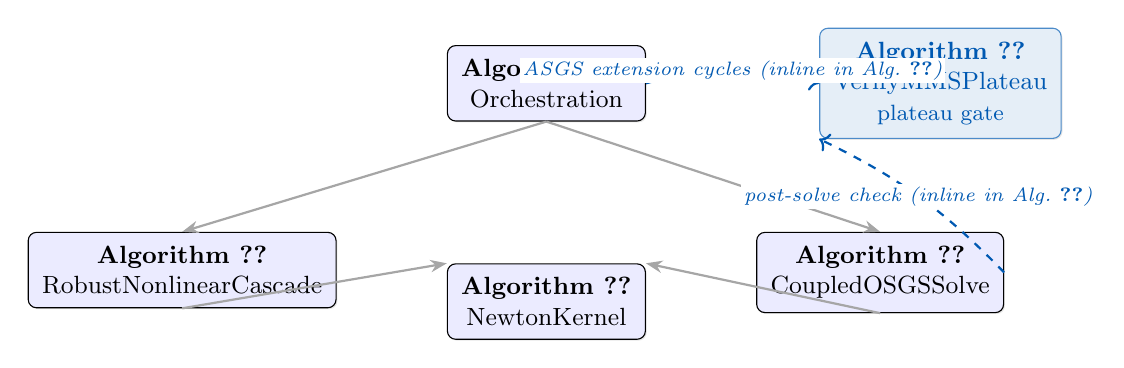
\begin{tikzpicture}[node distance=14mm and 10mm]

\node[modnode] (O)
    {\textbf{Algorithm~\ref{alg:O}}\\$\mathrm{Orchestration}$};

\node[modnode, below left=14mm and 14mm of O] (B)
    {\textbf{Algorithm~\ref{alg:B}}\\$\mathrm{RobustNonlinearCascade}$};
\node[modnode, below right=14mm and 14mm of O] (C)
    {\textbf{Algorithm~\ref{alg:C}}\\$\mathrm{CoupledOSGSSolve}$};

\node[modnode, below=18mm of O] (A)
    {\textbf{Algorithm~\ref{alg:A}}\\$\mathrm{NewtonKernel}$};

\node[extnode, right=22mm of O] (D)
    {\extline{\textbf{Algorithm~\ref{alg:D}}}\\\extline{$\mathrm{VerifyMMSPlateau}$}\\
     \extline{\footnotesize plateau gate}};

\draw[edge] (O.south) -- (B.north);
\draw[edge] (O.south) -- (C.north);
\draw[edge] (B.south) -- (A.north west);
\draw[edge] (C.south) -- (A.north east);

\draw[->, extcolor, thick, dashed]
    (O.east) to[bend left=15]
    node[edgelbl, midway, fill=white, text=extcolor]
    {\extline{ASGS extension cycles (inline in Alg.~\ref{alg:O})}} (D.west);
\draw[->, extcolor, thick, dashed]
    (C.east) to[bend right=10]
    node[edgelbl, midway, fill=white, text=extcolor]
    {\extline{post-solve check (inline in Alg.~\ref{alg:C})}} (D.south west);

\end{tikzpicture}
\caption{Extension hierarchy. The MMS plateau verifier
(\extline{Algorithm~\ref{alg:D}}, blue) is hooked directly into the
core orchestrator (Algorithm~\ref{alg:O}) and the core coupled OSGS
solve (Algorithm~\ref{alg:C}) by inline \extline{\textbackslash extline\{\}}
blue lines, displayed within the respective core algorithm boxes
(§\ref{sec:mms-hooks}). Solid arrows reproduce the core hierarchy of
Figure~\ref{fig:hierarchy}; \extline{dashed coloured arrows} mark the
extension hooks.}
\label{fig:ext-hierarchy}
\end{figure}

\section{Method of Manufactured Solutions Plateau Verifier}
\label{sec:mms}

\subsection{When this extension fires}

This extension is active whenever the solver is supplied with a
configuration \code{mms\_cfg} whose \code{enabled} flag is true. The
\code{mms\_cfg} object carries an analytical reference solution
$U_{\mathrm{exact}} = (\boldsymbol{u}_{\mathrm{ex}}, p_{\mathrm{ex}})$
(via an \code{oracle} callback) and a small set of plateau-test
parameters. When \code{mms\_cfg} is absent or disabled, the core
orchestration runs unchanged.

\subsection{Numerical versus discretisation convergence}

The inner Newton stops when $\|\boldsymbol{b}\|_\infty \le \textftol$.
That is convergence in the \emph{algebraic} sense: the iterate is
close to the root of the discrete system. It says nothing about
whether the discrete system is close to the true PDE solution. The
Method of Manufactured Solutions (MMS) provides exactly that second
test: it injects an exact analytical
$(\boldsymbol{u}_{\mathrm{ex}}, p_{\mathrm{ex}})$, recomputes the
appropriate source terms, and measures $\|U_h - U_{\mathrm{ex}}\|$ in
physical norms. The expected discretisation behaviour is $O(h^{k+1})$
in the $L^2$ norms (one order weaker in the $H^1$-semi norm).

For a single mesh, plateau verification asks a different question:
once the iterate is close enough to the root that further iterations
do not move the FE error, the FE error has \emph{plateaued} at its
discretisation floor.

\subsection{Algorithm D and its interface}

\extline{Algorithm~\ref{alg:D} is itself a leaf---a single side-by-side
comparison of consecutive FE errors against the exact solution. It
does not advance the iterate.}

\begin{tcolorbox}[colback=extcolor!5!white, colframe=extcolor, boxrule=0.4pt, arc=2pt, left=8pt, right=8pt, top=4pt, bottom=4pt, width=\textwidth, before skip=4pt, after skip=2pt]
\footnotesize
\extline{%
\begin{tabular}{@{}r@{\quad}p{0.82\textwidth}@{}}
\textit{Called by:} & The \code{SolutionVerifier} hooks the core invokes at each convergence point: \code{on\_asgs\_converged!} from Algorithm~\ref{alg:O} (per extension cycle in the ASGS path) and \code{on\_osgs\_converged!} from Algorithm~\ref{alg:C} (once, after the single coupled OSGS solve). The production path passes a no-op \code{NoVerification}; the MMS harness passes \code{MMSPlateauVerifier}. See §\ref{sec:mms-hooks}. \\
\textit{Calls:}     & (none; pure procedure) \\
\textit{Inputs:}    & Current iterate $U_h^m$; exact reference $U_{\mathrm{ex}}$; running error history $\mathcal{H}$; pass counter $I_{\mathrm{pass}}$ \\
\textit{Outputs:}   & Plateau flag $S_{\mathrm{plat}}$; updated counter $I_{\mathrm{pass}}'$ \\
\end{tabular}}
\end{tcolorbox}

\begin{algorithm}[H]
\caption{\extline{$\mathrm{VerifyMMSPlateau}$: relative-change plateau test (optional extension).}}
\label{alg:D}
\SetAlgoLined
\textcolor{extcolor}{\textbf{Parameters:} $N_{\mathrm{plat}}, \tau_{\mathrm{err}}, \varepsilon_{u,L^2}, \varepsilon_{u,H^1}, \varepsilon_{p,L^2}$.\\
\KwIn{$U_h^m$, $U_{\mathrm{ex}}$, $\mathcal{H}$, $I_{\mathrm{pass}}$.}
\KwOut{$(S_{\mathrm{plat}}, I_{\mathrm{pass}}')$.}
\vspace{0.2cm}\hrule\vspace{0.2cm}
compute $E_{u,L^2}^m$, $E_{u,H^1}^m$, $E_{p,L^2}^m$\;
append to $\mathcal{H}$; let $E^{m-1}_\bullet$ be the previous entry\;
$r_\bullet \gets |E_\bullet^m - E_\bullet^{m-1}| / \max(E_\bullet^m, E_\bullet^{m-1}, \varepsilon_\bullet)$ for each norm\;
$r_{\max} \gets \max_\bullet r_\bullet$\;
\If{$r_{\max} \le \tau_{\mathrm{err}}$}{
    $I_{\mathrm{pass}} \gets I_{\mathrm{pass}} + 1$\;
}\Else{
    $I_{\mathrm{pass}} \gets 0$\;
}
\If{$I_{\mathrm{pass}} \ge N_{\mathrm{plat}}$}{
    \Return $(\mathrm{True}, I_{\mathrm{pass}})$ \tcp*{plateau satisfied}
}
\Return $(\mathrm{False}, I_{\mathrm{pass}})$ \tcp*{continue extending}}
\end{algorithm}

\extline{The verifier tracks three error quantities, not two: $L^2$
of velocity, $L^2$ of pressure, and the $H^1$-semi-norm of velocity.
The third matters because the $L^2$ errors can plateau while the
velocity gradient---which is what the convective and viscous terms
actually feel---still drifts. The plateau is declared only after
$N_{\mathrm{plat}}$ \emph{consecutive} passes, and the counter resets
to zero on the first failure.}

\subsection{How Algorithm D hooks into the core}
\label{sec:mms-hooks}

\extline{The MMS plateau verifier is wired into the core algorithms by
two short blocks of conditional logic, displayed inline in
Algorithm~\ref{alg:O} (Stage~II dispatch) and Algorithm~\ref{alg:C}
(post-$S_{\mathrm{conv}}$ branch) and typeset in this colour. The
core path is recovered byte-for-byte by deleting every coloured line.}

\extline{In the ASGS branch of Algorithm~\ref{alg:O}, when
\code{mms\_cfg.enabled} is true, the orchestrator enters a bounded
plateau loop: up to $K_{\mathrm{extra}}$ extra single-Newton-step cycles
are run on top of the converged $U_h^{\mathrm{ASGS}}$, each followed
by a call to Algorithm~\ref{alg:D}. The loop exits as soon as the
plateau condition is satisfied or the budget is exhausted.}

\extline{In the OSGS branch, there is no plateau loop: the coupled solve
of Algorithm~\ref{alg:C} runs once and the MMS oracle is evaluated a
single time at its converged iterate $U_h^\star$. The orchestrator still
inflates the coupled-solve Newton budget
($N_{\mathrm{OSGS}}^{\mathrm{eff}} \gets N_{\mathrm{OSGS}} + K_{\mathrm{extra}}$),
but only to give the single solve extra inner-Newton room; the post-solve
hook records \code{mms\_stop\_reason} $=$ \code{coupled\_single\_solve} and,
if the velocity $L^2$ error exceeds the expected $O(h^{k_v+1})$ rate,
additionally records \code{coupled\_at\_suboptimal\_rate}. No extra
cycles are run and Algorithm~\ref{alg:D}'s consecutive-pass machinery
applies only to the ASGS extension path.}

\extline{\paragraph{What one $\mathcal{H}$-entry costs.}
In the ASGS extension loop, Algorithm~\ref{alg:D} compares the last two
entries of the running error history $\mathcal{H}$, each of which
corresponds to one extra \emph{single-Newton-step} on top of the
already-converged $U_h^{\mathrm{ASGS}}$. The plateau tolerance
$\tau_{\mathrm{err}}$ is calibrated against the relative change between
consecutive entries. The OSGS path takes no consecutive samples: it
evaluates the oracle once after the coupled solve, so $\tau_{\mathrm{err}}$
and the consecutive-pass count $N_{\mathrm{plat}}$ play no role there.}

\extline{\paragraph{The OSGS post-solve check is not a verification gate
on the solver.} The single OSGS oracle evaluation classifies the
converged FE error against the $O(h^{k_v+1})$ rate but does not gate
success: the coupled solve reports its own algebraic convergence, and the
\code{coupled\_at\_suboptimal\_rate} flag is a diagnostic recorded
alongside \code{mms\_stop\_reason} $=$ \code{coupled\_single\_solve}, not
a failure. Callers that care about FE-error verification must read those
diagnostics explicitly: a converged solver flag means the algebraic
system was solved, not that the discretisation error attained its optimal
rate. Treating $S_{\mathrm{solver}}$ alone as ``overall verification
success'' is a misuse of the return contract.}

\subsection{Parameters of this extension}

\begin{table}[h]
\centering
\caption{\extline{Numerical parameters of the MMS plateau verifier (extension-only).}}
\label{tab:mms-params}
\footnotesize
\textcolor{extcolor}{%
\begin{tabularx}{\textwidth}{@{} l l X @{}}
\toprule
\textbf{Symbol} & \textbf{Field in code} & \textbf{Role / effect} \\
\midrule
$N_{\mathrm{plat}}$ & \code{mms.require\_consecutive\_passes} & Consecutive passes of $r_{\max} \le \tau_{\mathrm{err}}$ required before declaring a plateau. \\
$\tau_{\mathrm{err}}$ & \code{mms.tau\_err} & Relative-change tolerance against which $r_{\max}$ is tested. \\
$\varepsilon_{u,L^2}, \varepsilon_{u,H^1}, \varepsilon_{p,L^2}$ & \code{mms.eps\_u\_l2,\_u\_h1,\_p\_l2} & Per-norm floors guarding the denominator in $r_{\max}$. \\
$K_{\mathrm{extra}}$ & \code{mms.max\_extra\_cycles} & Cap on extension cycles (ASGS path) or inner-Newton iterations added to the coupled-solve budget (OSGS path) for plateau verification. \\
\bottomrule
\end{tabularx}}
\end{table}

\section{Scale-free convergence criterion}
\label{sec:convergence-criterion}

\subsection{Motivation}
The stopping tests used elsewhere in Part~\ref{part:core} decide convergence relative to a scale that
is, in one way or another, supplied rather than measured: the scalar
$\|\boldsymbol{b}\|_\infty \le \textftol$ of Algorithm~\ref{alg:A} presumes all residual components
share one magnitude, and the harness per-field rule of Sec.~\ref{sec:harness-perfield} re-anchors the
target to the \emph{initial} residual $\|\boldsymbol{R}_0\|$, which drifts with the iterate once the
inner solve is split into Newton$\leftrightarrow$Picard segments. This section specifies a criterion
whose normalisation is \emph{measured from the current iterate and the known material data alone}, so
it is dimensionless and regime-robust with no a-priori characteristic velocity $U$, length $L$,
pressure $P$, or global $\mathrm{Re}$/$\mathrm{Da}$. It is realised as the standalone module
\code{src/solvers/convergence\_criterion.jl}, deliberately kept apart from the iteration machinery: it
answers \emph{whether} an iterate is converged, not \emph{how} to step. The full design rationale and a
critical audit of it live in \code{docs/solver/nonlinear-convergence-criterion-prompt.md}.

\subsection{The criterion}
With the momentum and mass residuals of the strong problem~\eqref{eq:alg-Ru}--\eqref{eq:alg-Rp}
evaluated at the iterate $U^k=(\boldsymbol{u}^k,p^k)$, the outer loop stops when
\begin{equation}
    \label{eq:cc-converged}
    \varepsilon_M \le \mathrm{tol}_M \quad\text{and}\quad \varepsilon_C \le \mathrm{tol}_C ,
\end{equation}
for the dimensionless momentum measure $\varepsilon_M$ and mass measure $\varepsilon_C$ below; both are
reported separately each iteration, alongside the per-term breakdown of $D_M$ (the diagnostic that
reveals which force balance is limiting a stalled solve).

\subsection{Momentum: the term-magnitude envelope}
\begin{equation}
    \label{eq:cc-epsM}
    \varepsilon_M = \frac{\|\boldsymbol{r}_M^k\|}{D_M^k}, \qquad
    D_M^k = \|\alpha\,\boldsymbol{u}^k\!\cdot\!\nabla\boldsymbol{u}^k\|
          + \|2\nabla\!\cdot\!(\alpha\nu\,\Pi^{\mathrm{ds}}\nabla\boldsymbol{u}^k)\|
          + \|\alpha\nabla p^k\|
          + \|\sigma(\alpha,\boldsymbol{u}^k)\,\boldsymbol{u}^k\|
          + \|\boldsymbol{f}\| ,
\end{equation}
the residual normalised by a dynamic envelope of the five momentum force magnitudes (convection,
viscous, pressure-gradient, Darcy--Forchheimer resistance, body force). At the solution these terms do
not vanish---they balance---so whichever mechanism dominates (viscous as
$\mathrm{Re},\mathrm{Da}\to0$, convection as $\mathrm{Re}\to\infty$, resistance as
$\mathrm{Da}\to\infty$) automatically enters the sum and sets the scale, with no regime parameter to
choose. The envelope is recomputed each iteration: $\sigma=a(\alpha)+b(\alpha)|\boldsymbol{u}^k|$ is
read pointwise from the iterate, and $\boldsymbol{f}$ is included because in forced problems it is one
of the balanced forces and can dominate.

\paragraph{Weak-form (algebraic) realisation.} The numerator $\boldsymbol{r}_M^k$ is the
\emph{stabilised} algebraic residual the solver actually drives to zero (the assembled ASGS/OSGS
residual vector, velocity block), and each denominator term is assembled through the \emph{same} weak
form with the same (Euclidean) vector norm. The viscous term is then the integrated-by-parts
first-derivative quantity
$\langle\boldsymbol{\varepsilon}^s(\boldsymbol{v}),\,2\alpha\nu\,\Pi^{\mathrm{ds}}\nabla\boldsymbol{u}^k\rangle$
(\code{weak\_viscous\_operator}); no second derivative appears, so the construction needs no
special-casing by polynomial order and is valid for the equal-order $P_{k_v}/P_{k_p}$ pair. Two
properties follow: (i) $\varepsilon_M\to0$ at the discrete solution---it reports genuine convergence
rather than plateauing at the $O(h^{k_v})$ floor of the \emph{strong} residual; and (ii) the
sum-of-norms is a conservative envelope, $D_M^k \ge \|\sum_i \mathrm{term}_i\|$, so cancellation between
co-dominant terms can never make $\varepsilon_M$ optimistically small. With consistent assembly
$\varepsilon_M\in[0,1]$ up to the bounded stabilisation contribution; a \emph{persistent}
$\varepsilon_M\gg1$ indicates the residual and the term decomposition were assembled inconsistently
(different quadrature/space/sign), not that the flow diverged.

\subsection{Mass: residual over a term-magnitude envelope}
\begin{equation}
    \label{eq:cc-epsC}
    \varepsilon_C = \frac{\bigl\|\,R_p^k\,\bigr\|}
                         {\|\nabla(\alpha\boldsymbol{u}^k)\|_F + \|g\|},
    \qquad
    R_p^k = \varepsilon\,p^k + \nabla\!\cdot\!(\alpha\boldsymbol{u}^k) - g ,
    \quad
    \nabla(\alpha\boldsymbol{u}^k)=\alpha\nabla\boldsymbol{u}^k
        + \boldsymbol{u}^k\!\otimes\!\nabla\alpha .
\end{equation}
The numerator is the \emph{genuine mass-equation residual} $R_p^k$: it subtracts the mass source
$g$ (the continuity forcing; $g\equiv0$ for the unforced physical problem, $g\neq0$ for a manufactured
solution with a non-solenoidal flux). Without the $-g$ term the ratio would measure the raw flux
divergence, which at the discrete solution equals the (nonzero) source and so floors at
$\|g\|/\|\nabla(\alpha\boldsymbol{u})\|$ instead of $\to0$, making it useless as a convergence gate on
a forced problem. The denominator is a mass-equation \emph{term-magnitude envelope}, exactly analogous
to the momentum $D_M$ (which carries the body force $\|f\|$): the robust flux-variation scale
$\|\nabla(\alpha\boldsymbol{u}^k)\|_F$ \emph{plus} the source magnitude $\|g\|$, so a strongly forced
mass equation is normalised by a scale that reflects its forcing. The Frobenius flux gradient stands
in for the divergence $\|\nabla\!\cdot\!(\alpha\boldsymbol{u})\|$ (which can collapse for a
near-incompressible flow) because boundary-layer shear keeps it bounded away from zero. All norms are
global $L^2(\Omega)$, built only from $\boldsymbol{u}^k$, $p^k$ and the known fields $\alpha$, $g$. The
penalty term $\varepsilon p^k$ is retained for strictness (negligible at the production
$\varepsilon\sim10^{-4}$). For constant $\alpha$, $\varepsilon=0$, $g=0$ it reduces to the textbook
$\|\nabla\!\cdot\!\boldsymbol{u}\|/\|\nabla\boldsymbol{u}\|$.

\paragraph{The $\sqrt{d}$ bound (and self-check).} The bound applies to the \emph{pure-divergence
ratio} $\|\nabla\!\cdot\!(\alpha\boldsymbol{u})\|/\|\nabla(\alpha\boldsymbol{u})\|_F$ (neither the
$g$-subtracted numerator nor the $g$-augmented denominator of $\varepsilon_C$ is $\sqrt{d}$-bounded).
Because $\nabla\!\cdot\!\boldsymbol{q}=\operatorname{tr}(\nabla\boldsymbol{q})$ and, by
Cauchy--Schwarz, $(\operatorname{tr}A)^2=(A:I)^2\le(A:A)(I:I)=d\,(A:A)$ pointwise, integration gives
$\|\nabla\!\cdot\!\boldsymbol{q}\|^2\le d\,\|\nabla\boldsymbol{q}\|_F^2$, so that ratio is
$\le\sqrt{d}$ in exact arithmetic. The criterion computes it separately as a cheap correctness check:
on a developed iterate a value above $\sqrt{d}$ flags a quadrature/assembly bug. It is \emph{logged as
a warning, not asserted}---in the degenerate roundoff regime the signed divergence sum can suffer
catastrophic cancellation and nudge the computed ratio slightly past $\sqrt{d}$ without any real
defect.

\subsection{Why it is scale-free, and what it is not}
The mass ratio is the pressure-normalised relative mass error with the divergence$\to$pressure
conversion factor \emph{measured from the iterate}: writing $\Phi/\alpha_\infty$ for the
viscous+inertial+Darcy envelope, steady-state balance gives $\|p^k\|\sim(\Phi/\alpha_\infty)\,
\|\nabla(\alpha\boldsymbol{u}^k)\|$, and substituting the measured
$\Phi/\alpha_\infty=\|p^k\|/\|\nabla(\alpha\boldsymbol{u}^k)\|$ into
$(\Phi/\alpha_\infty)\,\|\nabla\!\cdot\!(\alpha\boldsymbol{u}^k)\|/\|p^k\|$ cancels $\|p^k\|$
identically and leaves the flux-gradient denominator of~\eqref{eq:cc-epsC}; the added $\|g\|$ is a
known forcing field (material/problem data, not an a-priori characteristic scale), so it preserves
scale-freeness. The conversion factor carries units---that is what a
conversion does---while the surviving ratio is dimensionless because $\nabla\!\cdot$ and $\nabla$ of
the same field differ by exactly one inverse length. A pressure-referenced variant
$\varepsilon_C^{\mathrm{alt}}=\|(h^2/\alpha_K\tau_{1,K})\,\nabla\!\cdot\!(\alpha\boldsymbol{u}^k)\|/\|p^k\|$
is deliberately \emph{not} used: it divides by $\|p^k\|$, which is indeterminate under all-Dirichlet
velocity boundaries (pressure fixed only up to a constant) and is mesh-coupled through $\tau_1$ ---
strictly inferior to the genuinely scale-free~\eqref{eq:cc-epsC}.

\subsection{Edge cases and implementation guards}
\begin{itemize}
    \item \textbf{Trivial / degenerate iterate.} Every denominator is guarded by a pure machine-$\varepsilon$
    underflow floor (\emph{not} a problem scale); a denominator sitting at that floor raises a
    \code{degenerate} flag, and convergence is never accepted at $k=0$ (require $\ge1$ completed
    iteration). The $\sqrt{d}$ bound keeps $\varepsilon_C$ well-posed whenever
    $\|\nabla(\alpha\boldsymbol{u}^k)\|$ is above roundoff; the \code{degenerate} flag plus the
    $k\ge1$ rule cover the roundoff regime that the analytic bound cannot.
    \item \textbf{Genuine nonlinear residual.} $\boldsymbol{r}_M^k$ is the re-assembled operator residual
    at $U^k$, never the inner linear-solve residual (which $\to0$ \emph{inside} each step and does not
    reflect outer convergence).
    \item \textbf{Tolerance floor.} $\varepsilon_M$ and $\varepsilon_C$ cannot fall below the level set
    by the discretisation and by $\varepsilon$; $\mathrm{tol}$ must sit above it.
\end{itemize}

\subsection{Relation to the harness criterion}
The discretisation-coupled scalar tolerance~\eqref{eq:dynamic-ftol} and the per-field intrinsic-scale
rule of Sec.~\ref{sec:harness-perfield} are the parameter-sweep harness's convergence machinery; they
key the algebraic target to $h$ and to the per-field initial residual, which is appropriate inside a
manufactured-solution sweep where those quantities are known. The criterion of this section is their
production-grade, a-priori-scale-free counterpart: it requires no manufactured solution, no $h$, and no
initial-residual anchor, basing the normalisation entirely on the iterate's own force balance and flux
structure.

\section{Parameter-Sweep Harness Adaptations}
\label{sec:harness}

\subsection{When this extension fires}

\extline{These adaptations are active only when the solver is driven by
the project's parameter-sweep harness, which wraps the core
\code{run\_simulation} pipeline in a triple loop over $\mathrm{Re}$,
$\mathrm{Da}$, and the mesh-resolution parameter. In an ad-hoc
\code{run\_simulation} call, none of these adaptations fires; the core
algorithm of Part~\ref{part:core} uses the static parameters of
Table~\ref{tab:params} verbatim. The harness changes parameter
\emph{values} only; the algorithm boxes themselves are unchanged, so
no $\mathrm{O}'$ or $\mathrm{B}'$ variants are needed.}

\subsection{Discretisation-coupled residual tolerance}
\label{sec:harness-ftol}

\extline{Two error scales matter in an FE method. The \emph{algebraic
error} is the distance between the iterate and the discrete root.
The \emph{discretisation error} is the distance between the discrete
root and the true PDE solution, which behaves as $O(h^{k_v+1})$.
The harness derives a discretisation-coupled scalar tolerance,}
\begin{equation}
    \label{eq:dynamic-ftol}
    \textcolor{extcolor}{\textftol^{\,\mathrm{dyn}}
    = \max\!\Bigl(\textftol^{\,\mathrm{static}},\
        \min(C_{\mathrm{ceil}},\ C_{\mathrm{sf}} \cdot h^{k_v+1}) \Bigr),}
\end{equation}
\extline{in which $C_{\mathrm{sf}}$ ties the algebraic target to the
discretisation rate; the ceiling $C_{\mathrm{ceil}}$ guards against
trivially loose targets on coarse meshes; and the outer $\max$ pins
the tolerance above the user-supplied $\textftol^{\,\mathrm{static}}$.
Quantity~\eqref{eq:dynamic-ftol} couples the inner-Newton residual
target to the mesh---including the single coupled OSGS solve of
Algorithm~\ref{alg:C} (Sec.~\ref{sec:osgs})---and sets the plateau target
of Algorithm~\ref{alg:D} (Sec.~\ref{sec:mms}); for the
algebraic convergence of the inner Newton kernel,
Sec.~\ref{sec:harness-perfield} replaces this scalar criterion with a
per-field intrinsic-scale rule that remains physically meaningful when
the regime varies by many orders of magnitude.}

\subsection{Per-field intrinsic-scale convergence for the inner Newton}
\label{sec:harness-perfield}

\extline{The scalar test $\|\boldsymbol{b}\|_\infty \le \textftol$ used
throughout Algorithms~\ref{alg:A} and~\ref{alg:A3} carries a hidden
dimensional assumption: it presumes that all components of the
residual share one common scale. For the saddle-point system
considered here, this is incorrect. The assembled residual contains
momentum rows whose dimensions are $[\mu\, U / L^{2}]$ alongside
continuity rows whose dimensions are $[U/L]$, with the two natural
scales $U$ and $\mu$ varying by many orders of magnitude across
$(\mathrm{Re}, \mathrm{Da})$ space. A scalar threshold meaningful for
one regime is either trivially satisfied or unattainable in another.
The harness therefore declares the inner convergence target as a
\emph{dimensionless rate per field}, $\varepsilon_{k}$, and resolves
it to an absolute per-iteration tolerance via a scale proxy derived
from the iterate itself.}

\extline{Let $\mathcal{B}_{u}, \mathcal{B}_{p} \subseteq \{1,\dots,N\}$
denote the free-DOF index sets of the velocity and pressure field
blocks (the consecutive multi-field style of Gridap; the construction
generalises verbatim to $K > 2$ fields). Define the per-block
inf-norms of the residual and the iterate,}
\begin{equation}
    \label{eq:per-field-norms}
    \textcolor{extcolor}{
    R_{k}(\boldsymbol{b}) := \|\boldsymbol{b}[\mathcal{B}_{k}]\|_{\infty},
    \qquad
    \mathcal{U}_{k}^{\mathrm{raw}}(\boldsymbol{x}) := \|\boldsymbol{x}[\mathcal{B}_{k}]\|_{\infty},
    \qquad k \in \{u, p\}.}
\end{equation}

\extline{The scale proxy $\mathcal{U}_{k}(\boldsymbol{x})$ used to
non-dimensionalise the tolerance is recovered from the iterate
itself; no externally supplied $U_{c}, P_{c}$ enter the solver
interface. When both blocks of the iterate have acquired a
non-trivial magnitude, the proxy is the block's own inf-norm. When
one block remains at zero (the canonical case being a zero-pressure
initial condition together with a moving velocity), the missing scale
is recovered from the other block via the Bernoulli dimensional
identity $[p] = [\rho U^{2}]$, which under the constitutive
$\rho \equiv 1$ assumption of the present formulation reduces to a
square or square root:}
\begin{equation}
    \label{eq:per-field-scale-resolve}
    \textcolor{extcolor}{
    \mathcal{U}_{k}(\boldsymbol{x}) :=
    \begin{cases}
        \mathcal{U}_{k}^{\mathrm{raw}}(\boldsymbol{x})
            & \text{if } \mathcal{U}_{u}^{\mathrm{raw}}>0 \ \text{and}\ \mathcal{U}_{p}^{\mathrm{raw}}>0, \\[2pt]
        \bigl(\mathcal{U}_{p}^{\mathrm{raw}}\bigr)^{1/2}
            & \text{if } k = u,\ \mathcal{U}_{u}^{\mathrm{raw}} = 0,\ \mathcal{U}_{p}^{\mathrm{raw}} > 0, \\[2pt]
        \bigl(\mathcal{U}_{u}^{\mathrm{raw}}\bigr)^{2}
            & \text{if } k = p,\ \mathcal{U}_{p}^{\mathrm{raw}} = 0,\ \mathcal{U}_{u}^{\mathrm{raw}} > 0, \\[2pt]
        0
            & \text{if } \mathcal{U}_{u}^{\mathrm{raw}} = \mathcal{U}_{p}^{\mathrm{raw}} = 0.
    \end{cases}}
\end{equation}

\extline{The Bernoulli surrogate is physically motivated: momentum
balance for an incompressible flow fixes the dimensional ratio
between dynamic pressure and the square of the velocity, so a
pressure scale alone determines a consistent velocity scale (and
\emph{vice versa}) even before either field has been fully resolved.
The all-zero corner case is the unique state in which no scale
information is available from the iterate; resolution of this corner
defers to the absolute floor below.}

\extline{The effective per-field tolerance, recomputed at every
accepted Newton iterate $\boldsymbol{x}^{(i)}$, is}
\begin{equation}
    \label{eq:per-field-effective-ftol}
    \textcolor{extcolor}{
    \tau^{\mathrm{F}}_{k}\!\bigl(\boldsymbol{x}^{(i)}\bigr)
    := \max\!\Bigl(\textftol^{\,\mathrm{static}},\
        \varepsilon_{k} \cdot \mathcal{U}_{k}\!\bigl(\boldsymbol{x}^{(i)}\bigr)\Bigr),}
\end{equation}
\extline{where $\textftol^{\,\mathrm{static}}$ is a static
machine-precision floor (set in the harness at $10\,\mathrm{eps}$,
i.e.\ approximately $2.2\times 10^{-15}$ for double precision) whose
only role is to prevent the formula from demanding tolerances below
floating-point round-off when the per-field product
$\varepsilon_{k}\cdot \mathcal{U}_{k}$ vanishes or becomes
sub-precision. The dimensionless rate $\varepsilon_{k}$ is chosen to track
the FE discretisation rate,}
\begin{equation}
    \label{eq:per-field-rate}
    \textcolor{extcolor}{
    \varepsilon_{u} = \varepsilon_{p} = C_{\mathrm{sf}} \cdot h^{k_{v}+1},}
\end{equation}
\extline{so that the algebraic error tolerated at termination is, in
\emph{dimensionless} units, a fixed fraction $C_{\mathrm{sf}}$ of the
expected $O(h^{k_{v}+1})$ FE discretisation error---independently of
the regime. The dimensional tolerance recovered through
\eqref{eq:per-field-effective-ftol} thereby scales linearly with the
intrinsic magnitude of the field, while the convergence criterion
itself remains a single regime-independent number.}

\extline{The convergence and noise-floor predicates referenced by
Algorithms~\ref{alg:A} and~\ref{alg:A3} are the block-wise rules}
\begin{equation}
    \label{eq:per-field-convergence}
    \textcolor{extcolor}{
    \rho_{\mathrm{F}}\!\bigl(\hat{\boldsymbol{b}}, \boldsymbol{x}^{(i)}\bigr)
        := \bigwedge_{k \in \{u,p\}}
            \Bigl[\,R_{k}(\hat{\boldsymbol{b}})
                \le \tau^{\mathrm{F}}_{k}\!\bigl(\boldsymbol{x}^{(i)}\bigr)\Bigr],
    }
\end{equation}
\begin{equation}
    \label{eq:per-field-noise}
    \textcolor{extcolor}{
    \rho_{\mathrm{N}}\!\bigl(\hat{\boldsymbol{b}}, \boldsymbol{x}^{(i)}\bigr)
        := \bigwedge_{k \in \{u,p\}}
            \Bigl[\,R_{k}(\hat{\boldsymbol{b}})
                \le \tau^{\mathrm{N}}_{k}\!\bigl(\boldsymbol{x}^{(i)}\bigr)\Bigr],
        \qquad \tau^{\mathrm{N}}_{k} := \max\!\Bigl(\textstag^{\,\mathrm{dyn}},
        \varepsilon_{k}^{\mathrm{N}} \cdot \mathcal{U}_{k}\!\bigl(\boldsymbol{x}^{(i)}\bigr)\Bigr),}
\end{equation}
\extline{with the noise-floor scalar floor $\textstag^{\,\mathrm{dyn}}$
taken from~\eqref{eq:dynamic-noise} below and the noise-floor rate
$\varepsilon_{k}^{\mathrm{N}} = n^{\mathrm{sf}}\,\varepsilon_{k}$
preserving the fixed safety margin $n^{\mathrm{sf}} > 1$ above the
convergence rate (Sec.~\ref{sec:harness-noise}). The honest-exit
gate that wraps every $\mathsf{NoiseFloor}$ exit
(Sec.~\ref{sec:falseEquiv}) is likewise block-wise:}
\begin{equation}
    \label{eq:per-field-honest}
    \textcolor{extcolor}{
    \rho_{\mathrm{HE}}\!\bigl(\hat{\boldsymbol{b}}, \boldsymbol{x}^{(i)}\bigr)
        := \bigwedge_{k \in \{u,p\}}
            \Bigl[\,R_{k}(\hat{\boldsymbol{b}})
                \le K_{\mathrm{nf}}\, \tau^{\mathrm{F}}_{k}\!\bigl(\boldsymbol{x}^{(i)}\bigr)\Bigr].}
\end{equation}

\extline{In the algorithm boxes of Part~\ref{part:core}, the scalar
tests $\|\boldsymbol{b}\|_{\infty}\le \textftol$ and
$\|\boldsymbol{b}\|_{\infty}\le \textstag$ are read, under this
extension, as the corresponding predicates~\eqref{eq:per-field-convergence}
and~\eqref{eq:per-field-noise}; with $\varepsilon_{k} = 0$ the
predicates collapse exactly to the scalar form, preserving the core
algorithm verbatim when the extension is inactive.}

\paragraph{Per-iteration refresh.}
\label{sec:harness-perfield-refresh}
\extline{The proxy $\mathcal{U}_{k}$ in~\eqref{eq:per-field-effective-ftol}
is re-evaluated from the current iterate at every accepted
line-search step, not from the initial guess and not from any running
maximum. The reason is symmetric:}
\begin{itemize}[topsep=0pt, itemsep=0pt]
\item \extline{An initial guess that overshoots the true field
magnitude would, if left frozen, hold the tolerance at a permanently
loose value as the iterate shrinks toward the solution.}
\item \extline{An initial guess that undershoots (in particular, a
zero IC for which the Bernoulli fallback resolves the proxy from a
partial scale) would, if left frozen, hold the tolerance at a
permanently tight and unreachable value as the iterate grows.}
\end{itemize}
\extline{Both pathologies are avoided by tracking
$\mathcal{U}_{k}(\boldsymbol{x}^{(i)})$ adaptively. The cost is one
$O(\dim\mathcal{B}_{k})$ inf-norm per field per accepted iterate---negligible against the Jacobian assembly and linear solve that
dominate each iteration. Because the scale proxy depends only on the
iterate, the algorithm requires no external $(U_{c}, P_{c})$
declaration and therefore makes no problem-specific assumption.}

\subsection{Adaptive noise floor}
\label{sec:harness-noise}

\extline{Linear-system conditioning grows as $\mathcal{O}(h^{-2})$ for
elliptic operators and is amplified by convective and reactive terms.
A static $\textstag$ appropriate on a coarse mesh becomes far above
the genuine round-off floor on a fine mesh. The harness scales}
\begin{equation}
    \label{eq:dynamic-noise}
    \textcolor{extcolor}{\textstag^{\,\mathrm{dyn}}
    = \min\!\Bigl(\textstag,\ \max(n^{\min},\ n^{\mathrm{base}} \cdot N^2 \cdot \max(1, \mathrm{Re}))\Bigr),}
\end{equation}
\extline{with the additional clamp
$\textstag^{\,\mathrm{dyn}} \gets \max(\textstag^{\,\mathrm{dyn}}, n^{\mathrm{sf}}\textftol^{\,\mathrm{dyn}})$
preserving the strict ordering
$\textstag^{\,\mathrm{dyn}} > \textftol^{\,\mathrm{dyn}}$.}

\subsection{Per-case Picard widening}
\label{sec:harness-picard}

\extline{In a $(\mathrm{Re}, \mathrm{Da}, h)$ sweep, the harness widens
the Picard iteration budget when a stiffness threshold is exceeded:}
\begin{equation}
    \textcolor{extcolor}{\begin{aligned}
    N_{\mathrm{P}}^{\,\mathrm{local}} &\gets N_{\mathrm{P}}, \\
    \text{if } \mathrm{Re} \ge \mathrm{Re}^{\mathrm{th}}: \quad
    N_{\mathrm{P}}^{\,\mathrm{local}} &\gets \max(N_{\mathrm{P}}^{\,\mathrm{local}}, N_{\mathrm{P}}^{\mathrm{Re}}), \\
    \text{if } \mathrm{Da} \ge \mathrm{Da}^{\mathrm{th}}: \quad
    N_{\mathrm{P}}^{\,\mathrm{local}} &\gets \max(N_{\mathrm{P}}^{\,\mathrm{local}}, N_{\mathrm{P}}^{\mathrm{Da}}).
    \end{aligned}}
\end{equation}

\subsection{Parameters of this extension}

\begin{table}[h]
\centering
\caption{\extline{Numerical parameters of the parameter-sweep harness adaptations (extension-only).}}
\label{tab:harness-params}
\footnotesize
\textcolor{extcolor}{%
\begin{tabularx}{\textwidth}{@{} l l X @{}}
\toprule
\textbf{Symbol} & \textbf{Field in code} & \textbf{Role / effect} \\
\midrule
$C_{\mathrm{ceil}}$, $C_{\mathrm{sf}}$ & \code{sol.dynamic\_ftol\_ceiling}, \code{\_spatial\_safety\_factor} & Clamps for the discretisation-coupled residual tolerance \eqref{eq:dynamic-ftol}, \S\ref{sec:harness-ftol}; $C_{\mathrm{sf}}$ also sets the per-field dimensionless rate \eqref{eq:per-field-rate}. \\
$\varepsilon_{k}$, $\varepsilon^{\mathrm{N}}_{k}$ & (built from $C_{\mathrm{sf}}$, $n^{\mathrm{sf}}$, $h$, $k_{v}$) & Dimensionless per-field convergence and noise-floor rates supplied to the inner Newton kernel as \code{relative\_ftol\_per\_field} and \code{relative\_stagnation\_noise\_floor\_per\_field}, \S\ref{sec:harness-perfield}. \\
$\textftol^{\,\mathrm{static}}$ & (harness-set: $10\,\mathrm{eps}$) & Static machine-precision floor of~\eqref{eq:per-field-effective-ftol}; prevents per-field tolerances from descending below floating-point round-off. The corresponding noise-floor floor used in~\eqref{eq:per-field-noise} is $\textstag^{\,\mathrm{dyn}}$ from~\eqref{eq:dynamic-noise}. \\
$n^{\mathrm{base}}, n^{\min}, n^{\mathrm{sf}}$ & \code{sol.condition\_noise\_floor\_*} & Adaptive noise-floor controls, \S\ref{sec:harness-noise}. \\
$\mathrm{Re}^{\mathrm{th}}, N_{\mathrm{P}}^{\mathrm{Re}}$ & \code{sol.dynamic\_picard\_re\_*} & Per-case Picard widening trigger and budget for high Reynolds. \\
$\mathrm{Da}^{\mathrm{th}}, N_{\mathrm{P}}^{\mathrm{Da}}$ & \code{sol.dynamic\_picard\_da\_*} & Per-case Picard widening trigger and budget for high Damk\"ohler. \\
$\mathrm{Re}^{\mathrm{th,N}}, N_{\mathrm{N}}^{\mathrm{Re}}$ & \code{sol.dynamic\_newton\_re\_*} & Per-case Newton widening trigger and budget for high Reynolds. Mirrors the Picard pair; landed 2026-05-19 (\code{fa8aaec}) to absorb the transient smoothing phase the corrected mode-aware divergence safeguard exposes when Newton has to backtrack through residual-landscape spikes at $\mathrm{Re} \ge \mathrm{Re}^{\mathrm{th,N}}$. \\
\bottomrule
\end{tabularx}}
\end{table}

\end{document}
